\chapter{Low-Code}
    \begin{displayquote} \centering
        \say{\textit{The future of coding is no coding at all.}} \\
        \hspace*{\fill}---Chris Wanstrath, Co-Founder, Github
    \end{displayquote}
    \vspace{1em}

    Πριν προχωρήσουμε στην περιγραφή της υλοποίησης της εφαρμογής είναι κρίσιμο να αναφερθούμε στην έννοια του χαμηλού κώδικα (low code). Ο χαμηλός κώδικας αποτελεί απάντηση στην ανάγκη για γρηγορότερη παραγωγή ποιοτικών εφαρμογών, μάλιστα επιτρέποντας σε χρήστες με περιορισμένες ή μηδενικές γνώσεις προγραμματισμού να συμμετέχουν ενεργά στη διαδικασία ανάπτυξης. Η έννοια αυτή συνδέεται στενά με τις παλαιότερες προσπάθειες αυτοματοποίησης της ανάπτυξης λογισμικού, όπως το Computer-Aided Software Engineering (CASE) και η Model-Driven Architecture (MDA), οι οποίες αποτέλεσαν τις θεωρητικές ρίζες του χαμηλού κώδικα.

    Στο κεφάλαιο αυτό, παρουσιάζονται οι βασικές αρχές, τα χαρακτηριστικά και τα πλεονεκτήματα της προσέγγισης αυτής, το ιστορικό υπόβαθρο, η έννοια του προγραμματιστή πολίτη (citizen developer), και γίνεται αναφορά σε δημοφιλείς Πλατφόρμες Ανάπτυξης Εφαρμογών σε Low-Code και στον τρόπο που αυτές έχουν αναδιαμορφώσει το τοπίο της ανάπτυξης λογισμικού, αποτελώντας τη βάση για την εφαρμογή που παρουσιάζεται στην παρούσα εργασία. Μια εξ' αυτών, η Mendix, είναι αυτή που έχει χρησιμοποιηθεί για την ανάπτυξη της εφαρμογής και θα αναλυθεί στο επόμενο κεφάλαιο.


    \section{Τι είναι ο χαμηλός κώδικας}
        \begin{displayquote} \justifying
            \say{\textit{When you can visually create new business applications with minimal hand-coding --when your developers can do more of greater value, faster-- that’s low-code.}} \cite{Ibm_2024}
        \end{displayquote}

        Για να κατανοήσουμε καλύτερα την έννοια του χαμηλού κώδικα, μπορούμε να εξετάσουμε την εξέλιξη των γλωσσών προγραμματισμού. Για παράδειγμα, η Python, μια γλώσσα υψηλού επιπέδου, θα μπορούσε να χαρακτηριστεί ως χαμηλός κώδικας σε σύγκριση με τη C++. Αντίστοιχα η C θα μπορούσε να χαρακτηριστεί και αυτή χαμηλός κώδικας συγκριτικά με την Assembly, όπως και η Assembly είναι χαμηλός κώδικας αν τη συγκρίνουμε με το να αλλάζουμε χειροκίνητα μηδενικά και άσσους στους καταχωρητές. Πρακτικά, η εξέλιξη του προγραμματισμού ταυτίζεται με την εξέλιξη του χαμηλού κώδικα.

        Επομένως, ο χαμηλός κώδικας, αν και ονομάστηκε πρόσφατα ως όρος, η \textit{έννοιά} του δεν είναι καθόλου καινούρια, και είναι η άμεση εξέλιξη του υψηλού επιπέδου γλωσσών προγραμματισμού (4GLs) των τελευταίων δεκαετιών. Το υψηλότερο προγραμματιστικό επίπεδο με τις αφαιρέσεις που διαθέτει, επιτρέπει ευκολότερη και γρηγορότερη ανάπτυξη λογισμικού. Πέρα όμως από τους χρήστες που είναι ήδη προγραμματιστές, προσφέρει επιπλέον τη δυνατότητα σε χρήστες με λίγη ή και καθόλου προγραμματιστική εμπειρία (προγραμματιστές πολίτες -- περιγράφονται αναλυτικότερα στο \ref{subsec:citizen-developer}). να τροποποιήσουν εφαρμογές ή και να φτιάξουν εξ' ολοκλήρου τις δικές τους, με την ίδια λογική όπως η Python επέτρεψε σε περισσότερο κόσμο να προγραμματίσει σε σχέση με την Assembly.

        Ο προγραμματισμός σε χαμηλό κώδικα πραγματοποιείται σε πλατφόρμες που ονομάζονται \textbf{Πλατφόρμες Ανάπτυξης Λογισμικού σε Low-Code} (Low-Code Development Platforms -- LCDPs), οι οποίες θα αναλυθούν στην ενότητα \ref{sec:LCDP}. Οι πλατφόρμες περιλαμβάνουν γραφικό περιβάλλον με drag-and-drop και WYSIWYG (What-You-See-Is-What-You-Get) editors, επιτρέποντας την πιο γρήγορη και ενστικτώδη κατασκευή εφαρμογών. Αυτός ο οπτικός προγραμματισμός (visual programming) είναι σημαντικός παράγοντας στην προσβασιμότητα που προσφέρει ο χαμηλός κώδικας. \cite{LowCodeMendix} \cite{LowCodeSimon} \cite{LowCodeDemocratization}

            \subsection{Οπτικός προγραμματισμός (visual programming)}
                Στο σχήμα \ref{fig:codevsmendix} παρατίθενται δύο παραδείγματα από την παραδοσιακή ανάπτυξη εφαρμογών και την ανάπτυξη εφαρμογών σε low-code στην πλατφόρμα Mendix.

                \begin{figure}[h!] \noindent
                        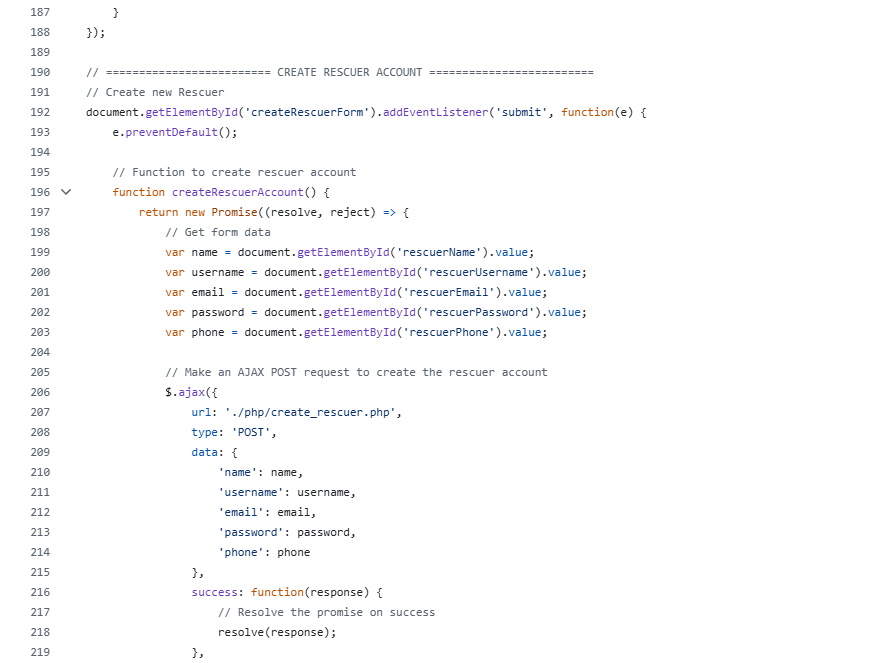
\includegraphics[trim={0 3cm 0 0}, clip, width=0.8\textwidth]{ClassicProgramming}
                        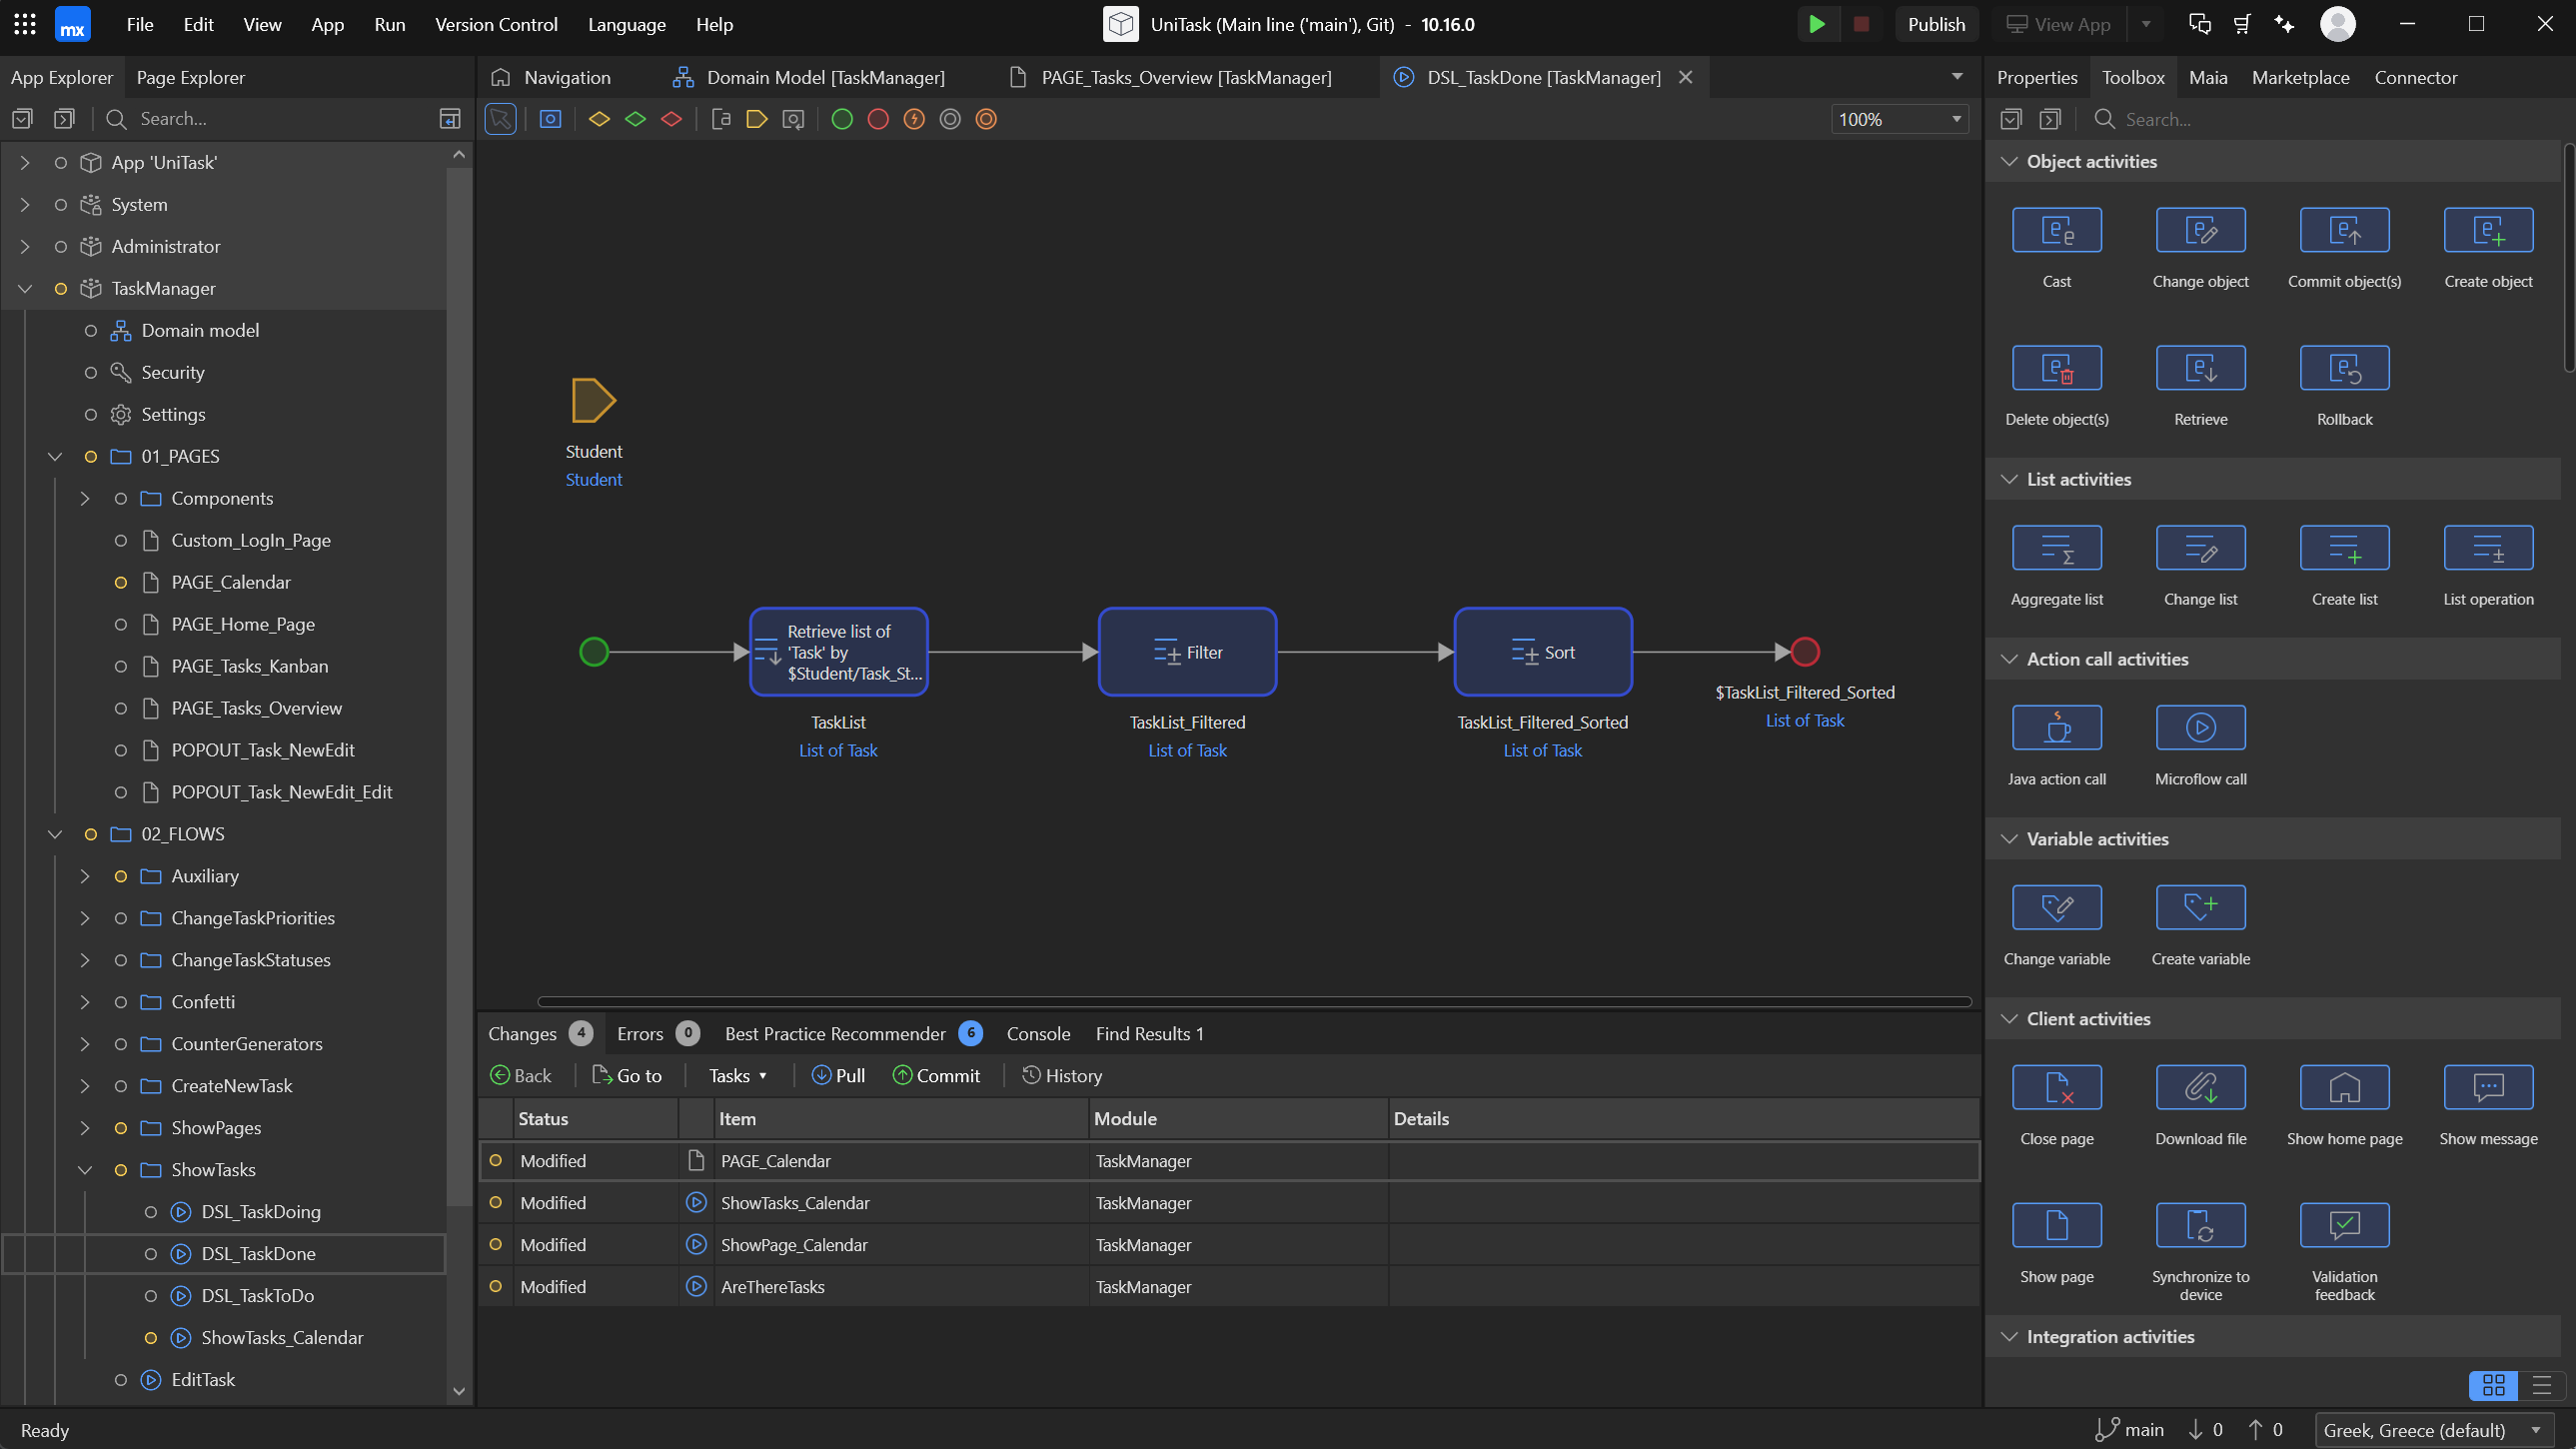
\includegraphics[width=\textwidth]{MendixLowCodeDevelopment}
                        \caption{Παραδοσιακός κώδικας και το γραφικό περιβάλλον του Mendix.}
                        \label{fig:codevsmendix}
                \end{figure}

                Στο γραφικό περιβάλλον, ο προγραμματισμός γίνεται σε ένα διάγραμμα ροής με drag-and-drop επαναχρησιμοποιούμενα στοιχεία. Αυτή η προσέγγιση διευκολύνει την ανάπτυξη εφαρμογών, καθώς επιτρέπει στους χρήστες να επικεντρωθούν στη λογική της εφαρμογής, χωρίς να χρειάζεται να ασχοληθούν με τη σύνταξη και τις λεπτομέρειες του κώδικα. Στο σχήμα \ref{fig:codevsmendix}, παρατηρούμε ένα χαρακτηριστικό παράδειγμα επαναχρησιμοποιούμενων στοιχείων· τα μπλε τετράγωνα στο διάγραμμα ροής αποτελούν βασικά δομικά συστατικά που μπορούν να τοποθετηθούν και να συνδεθούν εύκολα. Στη δεξιά πλευρά της οθόνης εμφανίζεται μια βιβλιοθήκη εργαλείων (toolbox), μέσω της οποίας οι χρήστες μπορούν να επιλέξουν και να προσθέσουν τα απαραίτητα στοιχεία στο διάγραμμά τους. Η διαδικασία αυτή, σε αντίθεση με την παραδοσιακή γραμμή-γραμμή σύνταξη κώδικα (υψηλός κώδικας), καθιστά την ανάπτυξη εφαρμογών εξαιρετικά γρήγορη, μειώνοντας τον χρόνο εκμάθησης και διευρύνοντας το φάσμα των χρηστών που μπορούν να συμμετάσχουν σε αυτήν.

                Η οπτικοποίηση του προγραμματισμού αποτελεί μια εκ θεμελίων επαναστατική αλλαγή, καθώς αναδεικνύει μια βαθιά ανθρώπινη ανάγκη: τη χρήση της οπτικής επικοινωνίας για την κατανόηση και τη μεταφορά ιδεών. Εξάλλου οι πρώτες πετρογραφίες και οι ζωγραφιές στους τοίχους των σπηλαίων αποδεικνύουν ότι η οπτική παράσταση ήταν ανέκαθεν ένα ισχυρό εργαλείο επικοινωνίας \cite{CASEKuhn}. Ο οπτικός προγραμματισμός στηρίζεται σε αυτή τη λογική και τη μεταφέρει στον σύγχρονο κόσμο της τεχνολογίας. Η χρήση του ποντικιού, το οποίο θεωρείται πιο προσιτό από το πληκτρολόγιο για τους περισσότερους χρήστες, διευκολύνει τη διαδικασία εισαγωγής, επεξεργασίας και διασύνδεσης στοιχείων. Το αποτέλεσμα είναι ένα περιβάλλον που συνδυάζει λειτουργικότητα και ευκολία, εξαλείφοντας την ανάγκη για εξειδικευμένες τεχνικές γνώσεις, ενώ ταυτόχρονα αυξάνει την αποδοτικότητα της ανάπτυξης.

                Τέλος, είναι σημαντικό να αναφερθεί πως η οπτική προσέγγιση επιτρέπει την ταχύτερη ανίχνευση σφαλμάτων και την πιο αποτελεσματική συνεργασία μεταξύ των μελών μιας ομάδας, καθώς ένα διάγραμμα ροής είναι άμεσα κατανοητό από όλους τους εμπλεκόμενους, ανεξαρτήτως τεχνικού υποβάθρου.

            \subsection{Καθόλου κώδικας (no-code)}
                Ένας εύληπτος τρόπος για να κατανοήσουμε τη διαφορά ανάμεσα στον χαμηλό κώδικα και τον καθόλου κώδικα είναι η προσέγγιση που ακολουθείται στην αλληλεπίδραση με το λογισμικό. Στα no-code περιβάλλοντα, οι χρήστες δε χρειάζεται να χρησιμοποιούν καθόλου το πληκτρολόγιο· όλες οι ενέργειες πραγματοποιούνται μέσω ποντικιού, αξιοποιώντας ένα πλήρως γραφικό περιβάλλον. Η διαδικασία αυτή εξαλείφει κάθε ανάγκη γραφής κώδικα, καθιστώντας τα no-code περιβάλλοντα ιδιαίτερα ελκυστικά για χρήστες που δε διαθέτουν τεχνικές γνώσεις.

                Ένα βασικό μειονέκτημα αυτών των συστημάτων είναι η έλλειψη ευελιξίας. Οι χρήστες δεν μπορούν να προσαρμόσουν πλήρως τις εφαρμογές στις ιδιαίτερες ανάγκες τους, καθώς αφού δεν υπάρχει η δυνατότητα για εξατομίκευση με custom κώδικα, οι χρήστες περιορίζονται αποκλειστικά από τις δυνατότητες που έχουν προκαθοριστεί από την πλατφόρμα. Από την άλλη, ο περιοριστικός χαρακτήρας αυτών των εργαλείων ελαχιστοποιεί την πιθανότητα εμφάνισης σφαλμάτων και έτσι αυξάνεται η απλότητα και η ακρίβεια.

                Αντίθετα, ο χαμηλός κώδικας (low-code) συνδυάζει τα καλύτερα στοιχεία και των δύο κόσμων: της παραδοσιακής προγραμματιστικής διαδικασίας και των no-code εργαλείων. Οι χρήστες μπορούν να αξιοποιήσουν την απλότητα και την ευκολία του γραφικού περιβάλλοντος, αλλά παράλληλα έχουν τη δυνατότητα να ενσωματώσουν τον δικό τους κώδικα για πλήρη παραμετροποίηση και ανάπτυξη. Αυτή η προσέγγιση καθιστά τα low-code εργαλεία ιδανικά για πιο σύνθετα έργα, όπου απαιτούνται πιο προσαρμοσμένες λύσεις. \cite{LowCodeSimon}

            \begin{figure}[h!] \noindent \centering
                    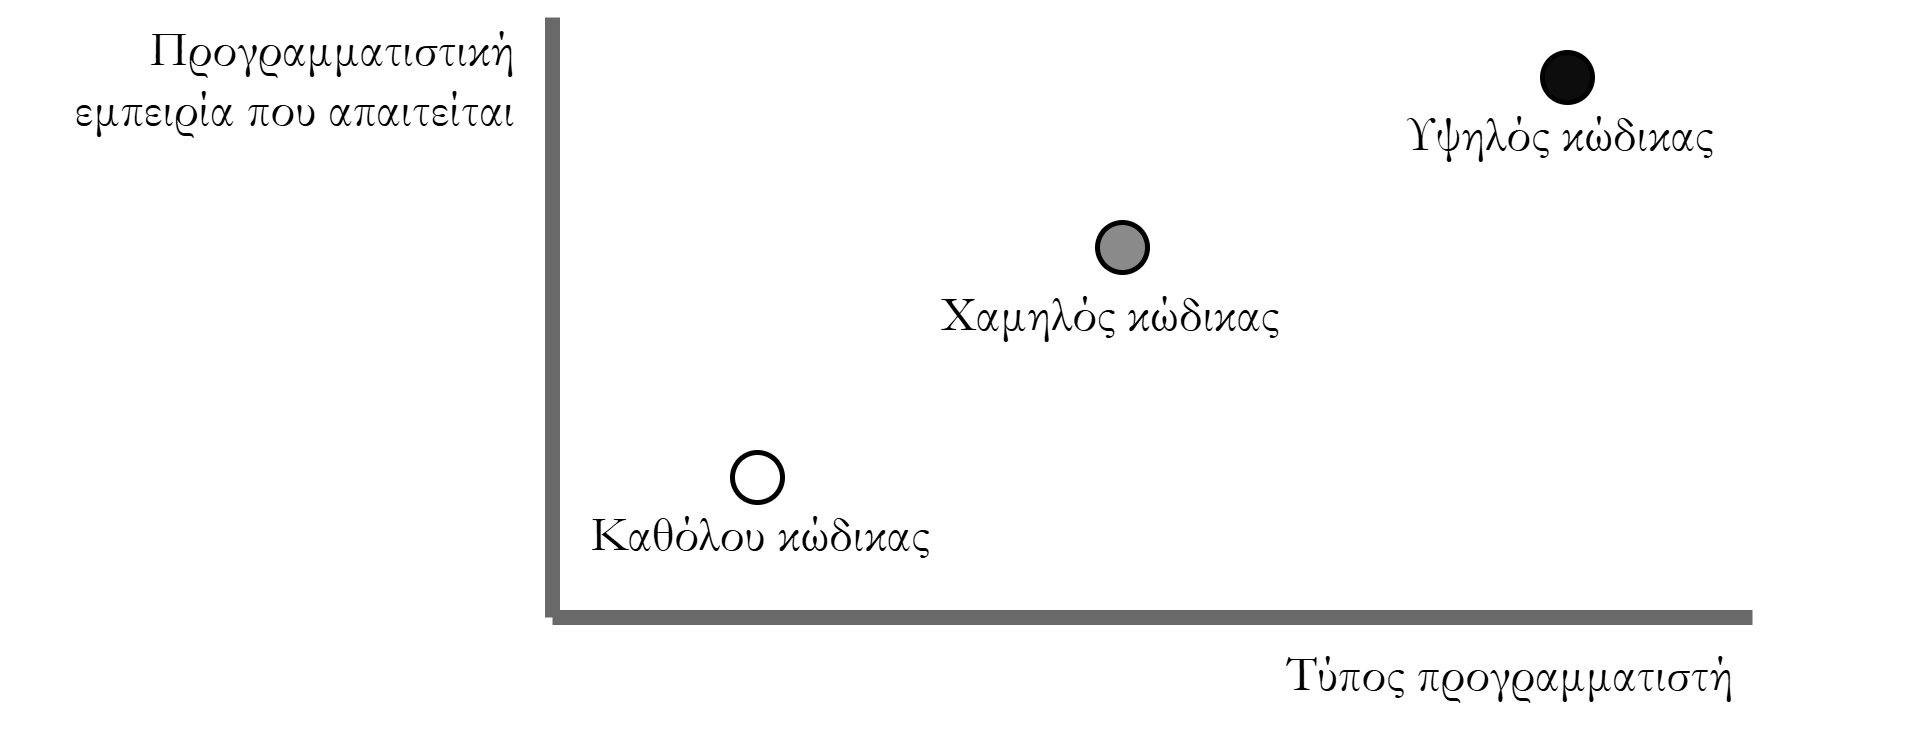
\includegraphics[width=0.9\textwidth]{diagrams/DeveloperVsCode_gr}
                    \caption{\centering Σύγκριση ανάμεσα στην προγραμματιστική εμπειρία των χρηστών \\ και την προγραμματιστική προσέγγιση που χρησιμοποιούν \cite{LowCodeSimon}}
            \end{figure}

            \subsection{Η έννοια του προγραμματιστή πολίτη (citizen developer)} \label{subsec:citizen-developer}
                Ο προγραμματιστής πολίτης είναι ένας χρήστης που αναπτύσσει εφαρμογές σε συνεργασία με τους προγραμματιστές, χωρίς να είναι απαραίτητο να διαθέτει προγραμματιστικές γνώσεις. Η έλλειψη προηγούμενων γνώσεων και εμπειρίας στον προγραμματισμό δεν τον εμποδίζει από το να συνεισφέρει στην ανάπτυξη με ισότιμο τρόπο όπως οι παραδοσιακοί προγραμματιστές.

                Μια περίληψη των βασικών διαφορών που παρατηρούνται ανάμεσα στους προγραμματιστές πολίτες και τους μηχανικούς λογισμικού συνοψίζεται στον παρακάτω πίνακα \cite{LowCodeSimon}:

                \begin{table}[H] \noindent\centering
                    \resizebox{\textwidth}{!}{
                        \begin{tabular}{c|c|c}
                           \textbf{Χαρακτηριστικό} & \textbf{Παραδοσιακός μηχανικός λογισμικού} & \textbf{Προγραμματιστής πολίτης} \\
                            \midrule
                            Γνωστικό & Μηχανική λογισμικού ή & Ποικίλει \\
                            υπόβαθρο & Επιστήμη των Υπολογιστών & \\
                            \midrule
                            Θέση στην & Τεχνολογία πληροφοριών (IT), & Μάρκετινγκ, πωλήσεις, \\
                            επιχείρηση & DevOps & HR, λογιστικά \\
                            \midrule
                            Γνώσεις που αφορούν & Λίγες & Πολλές \\
                            την επιχείρηση & & \\
                        \end{tabular}}
                \end{table}

                Ο ρόλος των προγραμματιστών πολιτών αναμένεται να γνωρίσει σημαντική άνοδο τα επόμενα χρόνια. Δεν πρόκειται τόσο για μια νέα εξειδικευμένη θέση εργασίας όσο για ένα πρόσθετο χαρακτηριστικό που θα ενσωματωθεί σε ήδη υπάρχουσες θέσεις. Οι εργαζόμενοι που αναλαμβάνουν διοικητικές, επιχειρηματικές ή άλλες λειτουργικές αρμοδιότητες θα αποκτούν δεξιότητες ανάπτυξης λογισμικού, επιτρέποντας τους να αναπτύσσουν λύσεις προσαρμοσμένες στις ανάγκες τους, χωρίς να εξαρτώνται αποκλειστικά από τις ομάδες προγραμματιστών.

                Η Gartner, μια κορυφαία διεθνής εταιρία ερευνών και συμβουλευτικών υπηρεσιών που εξειδικεύεται στους τομείς της τεχνολογίας, της επιχειρηματικής στρατηγικής και της καινοτομίας, υπογραμμίζει τη δυναμική αυτής της εξέλιξης. Σύμφωνα με έκθεσή της, προβλέπεται πως «έως το 2023, ο αριθμός των ενεργών προγραμματιστών πολιτών σε μεγάλες επιχειρήσεις θα είναι τουλάχιστον τετραπλάσιος από τον αριθμό των παραδοσιακών προγραμματιστών» \cite{GartnerReport}. Επίσης, σύμφωνα με φετινή έκθεσή της αναφέρεται πως «μέχρι το 2029, οι πλατφόρμες ανάπτυξης εφαρμογών low-code για επιχειρήσεις (Enterprise LCAPs) θα χρησιμοποιούνται για την ανάπτυξη εφαρμογών κρίσιμης σημασίας στο 80\% των επιχειρήσεων παγκοσμίως, σε σύγκριση με το 15\% που είναι το 2024». \cite{mendixGartnerQuadrant}

                Επιπλέον, η Microsoft ενισχύει αυτήν την πρόβλεψη, επισημαίνοντας ότι «μέχρι το 2025, οι προγραμματιστές πολίτες θα έχουν δημιουργήσει 450 εκατομμύρια εφαρμογές χρησιμοποιώντας πλατφόρμες χαμηλού ή καθόλου κώδικα» \cite{cnbcNextFrontier}. Αυτή η εντυπωσιακή αριθμητική αύξηση σηματοδοτεί μια νέα εποχή στον τρόπο με τον οποίο προσεγγίζεται η ανάπτυξη λογισμικού, δίνοντας έμφαση στη συμμετοχή ευρύτερων ομάδων εργαζομένων, ενώ παράλληλα αναδεικνύουν τον εκδημοκρατισμό της τεχνολογίας.

                \subsubsection{Διαφορά με τους παραδοσιακούς προγραμματιστές}
                    Οι παραδοσιακοί προγραμματιστές (προγραμματιστές υψηλού κώδικα), σε αντίθεση με την αρχική εντύπωση που μπορεί να δημιουργείται, δεν αντιμετωπίζουν τους προγραμματιστές πολίτες με καχυποψία ή φόβο για απώλεια του ρόλου τους. Αντίθετα, δείχνουν ενθουσιασμό για την παρουσία και την προσφορά τους. Ο λόγος πίσω από αυτή τη θετική στάση είναι απλός και συνοψίζεται στο σχήμα \ref{fig:DevVSCitDev}.

                    \begin{figure}[h!] \noindent \centering
                            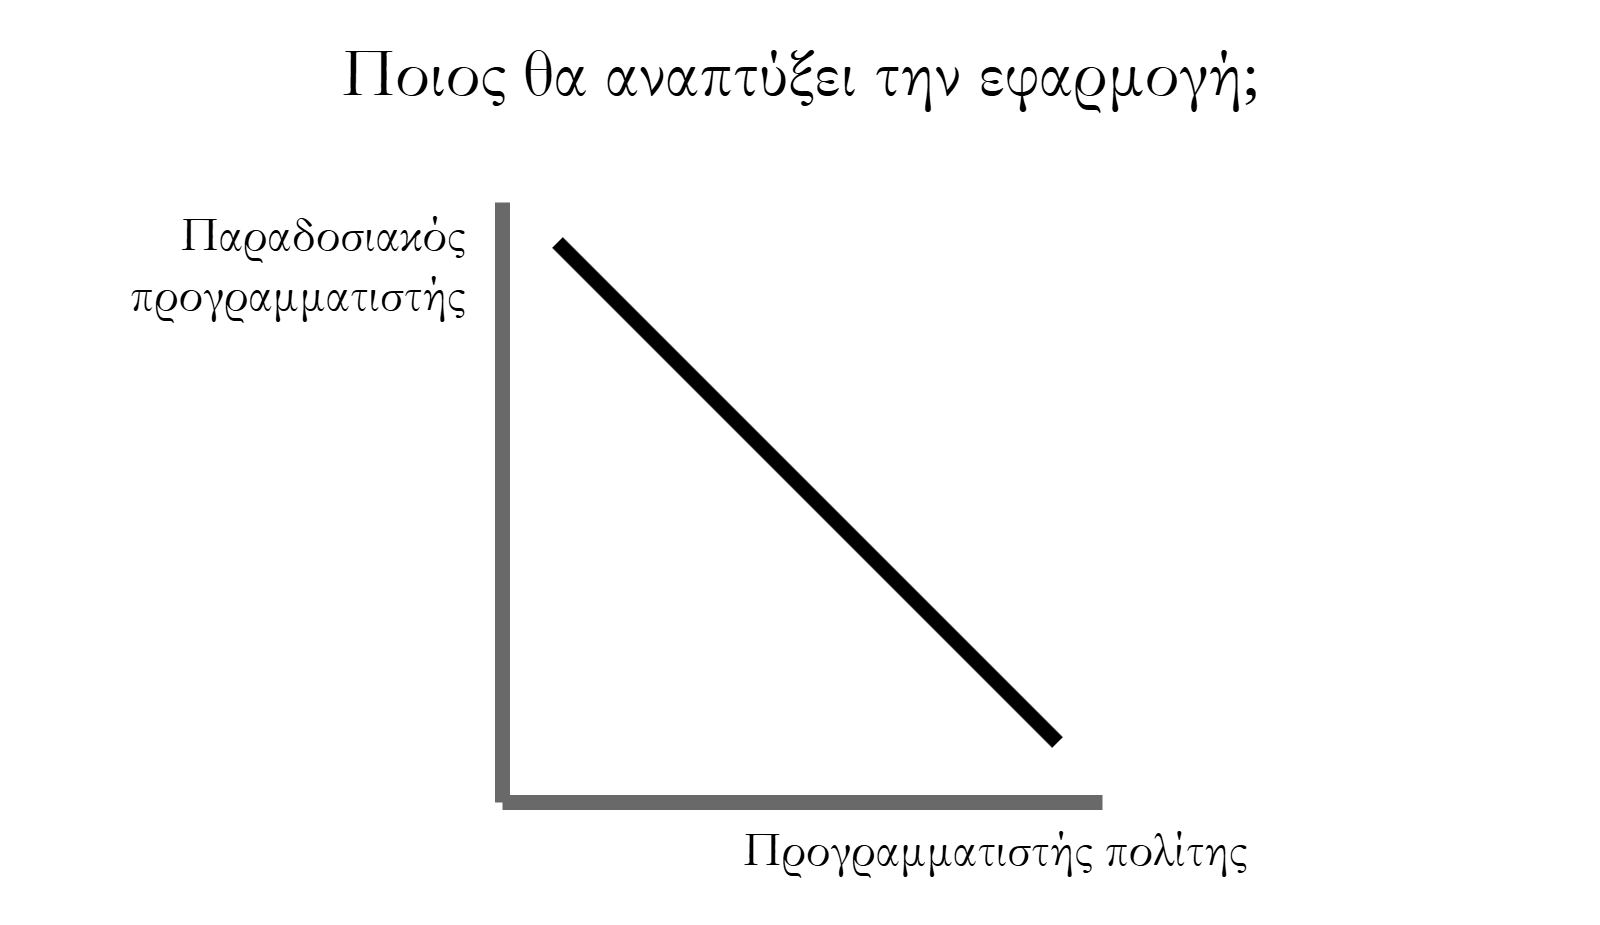
\includegraphics[width=0.7\textwidth]{diagrams/DevVSCitDev_gr}
                            \caption{Ποιος θα φτιάξει την εφαρμογή; \cite{LowCodeSimon}}
                            \label{fig:DevVSCitDev}
                    \end{figure}

                    Παρότι οι προγραμματιστές πολίτες μπορούν και \textit{συνεισφέρουν} στην υλοποίηση απλών εφαρμογών, παραμένει ανέφικτο για αυτούς να αναλάβουν τον σχεδιασμό και την ανάπτυξη πολύπλοκων συστημάτων που απαιτούν σχεδιαστική γνώση και εμπειρία. Αυτή η πραγματικότητα δημιουργεί έναν φυσικό διαχωρισμό ρόλων. Με ένα σημαντικό μέρος της εργασίας που σχετίζεται με καθημερινές, επαναλαμβανόμενες διαδικασίες να μεταφέρεται στους προγραμματιστές πολίτες, οι επαγγελματίες προγραμματιστές απελευθερώνονται από τα βάρη των «αδιάφορων» λεπτομερειών και μπορούν να αφιερώσουν περισσότερη ενέργεια στη σχεδίαση, την αρχιτεκτονική των εφαρμογών και σε πιο στρατηγικούς στόχους. Αυτό σημαίνει ότι αντί να ασχολούνται με λεπτομέρειες που μπορεί να διεκπεραιωθούν με τη βοήθεια εργαλείων χαμηλού ή καθόλου κώδικα, στρέφουν την προσοχή τους σε σύνθετα ζητήματα όπως η κλιμάκωση των συστημάτων, η διασφάλιση της ασφάλειας, η βελτιστοποίηση των επιδόσεων και η δημιουργία καινοτόμων λύσεων. \cite{Sahay2020}

                    Οι προγραμματιστές πολίτες και οι παραδοσιακοί προγραμματιστές μαζί συνθέτουν μια δυναμική ομάδα που καλύπτει ένα ευρύ φάσμα αναγκών, προάγοντας την αποτελεσματικότητα και την καινοτομία στην ανάπτυξη λογισμικού.

                \subsubsection{Χαρακτηριστικά των προγραμματιστών πολιτών}
                    Σε μια έρευνα που πραγματοποιήθηκε από την εταιρεία QuickBase \cite{QuickBaseCitizenDevReport}, στην οποία συμμετείχαν 148 αυτοαποκαλούμενοι προγραμματιστές πολίτες, αναδεικνύονται σημαντικά χαρακτηριστικά αυτής της ομάδας. Σύμφωνα με τα αποτελέσματα της έρευνας, το 97\% των συμμετεχόντων κατείχε βασικές δεξιότητες στη χρήση εργαλείων επεξεργασίας κειμένου και υπολογιστικών φύλλων, ενώ το 36\% των ερωτηθέντων διέθετε γνώσεις front-end web development, όπως HTML, CSS και JavaScript, επιβεβαιώνοντας ότι ορισμένοι προγραμματιστές πολίτες διαθέτουν τεχνικό υπόβαθρο πέρα από τα βασικά. Επιπλέον, ένα μικρότερο αλλά εξίσου σημαντικό ποσοστό, το 8\%, είχε επαφή με πιο προχωρημένες γλώσσες προγραμματισμού, όπως Java, .NET, Python, Ruby και PHP, δείχνοντας ότι οι δεξιότητες ορισμένων προγραμματιστών πολιτών επεκτείνονται και σε πιο παραδοσιακές τεχνολογίες ανάπτυξης λογισμικού.

                    \begin{figure}[h!] \noindent \centering
                            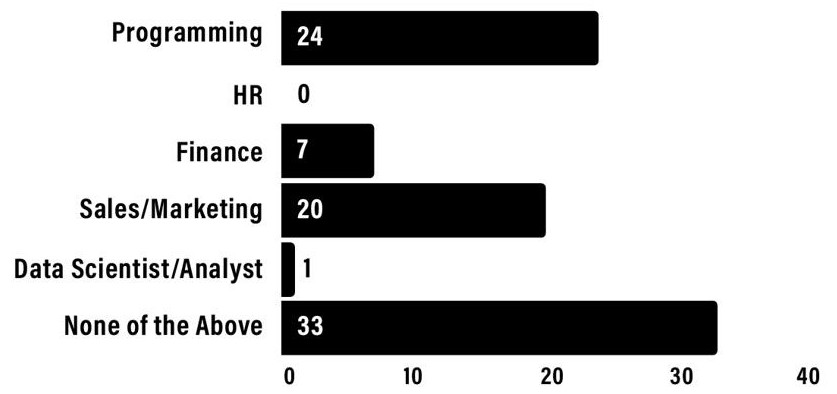
\includegraphics[width=0.6\textwidth]{CitDevBg}
                            \caption{Επαγγελματικό υπόβαθρο προγραμματιστών πολιτών. \cite{LowCodeSimon}}
                            \label{fig:CitDevBg}
                    \end{figure}

                    Το σχήμα \ref{fig:CitDevBg} παρουσιάζει έναν επιπλέον ενδιαφέρων διαχωρισμό: το 72\% των προγραμματιστών πολιτών δεν είναι επαγγελματίες προγραμματιστές, αλλά προέρχονται από διαφορετικά επαγγελματικά αντικείμενα. Από την άλλη πλευρά, το 28\% των συμμετεχόντων που είναι ήδη επαγγελματίες προγραμματιστές δείχνει μια τάση αποδοχής των εργαλείων χαμηλού και καθόλου κώδικα ακόμα και από αυτούς που έχουν την ικανότητα να γράφουν παραδοσιακό κώδικα. Τέλος, το σχήμα \ref{fig:CitDevAge} φανερώνει πως οι νεότερες γενιές εμφανίζουν αυξημένες πιθανότητες να ασχολούνται ως προγραμματιστές πολίτες. Αυτή η παρατήρηση μπορεί να αποδοθεί στη μεγαλύτερη εξοικείωση των νεότερων ηλικιακά με την τεχνολογία και τα ψηφιακά εργαλεία, καθώς και στη διάθεση για καινοτομία και πειραματισμό που χαρακτηρίζει τις γενιές αυτές. Επιπλέον, η αυξημένη διείσδυση εργαλείων χαμηλού κώδικα στην εκπαίδευση και στο επαγγελματικό περιβάλλον φαίνεται να ενθαρρύνει τη συμμετοχή νεότερων ατόμων, δημιουργώντας τις προϋποθέσεις για περαιτέρω διάδοση του φαινομένου.

                    \begin{figure}[h!] \noindent \centering
                            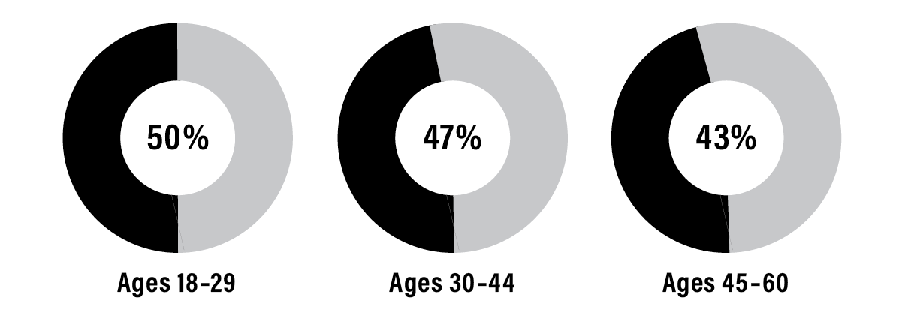
\includegraphics[width=0.7\textwidth]{CitDevAge}
                            \caption{Ηλικιακή κατανομή προγραμματιστών πολιτών. \cite{CitDevTrackVia}}
                            \label{fig:CitDevAge}
                    \end{figure}


    \section{Πώς φτάσαμε στον χαμηλό κώδικα}
        Πριν προχωρήσουμε στις Πλατφόρμες Ανάπτυξης Λογισμικού σε Low-Code, αξίζει να αναφερθούμε πρώτα στις τεχνολογικές εξελίξεις που μας οδήγησαν σήμερα στην ύπαρξη αυτών των πλατφορμών, ξεκινώντας με τον ορισμό της μηχανικής λογισμικού.

        Η μηχανική λογισμικού είναι ο τομέας που ασχολείται με τη συστηματική ανάπτυξη και διαχείριση υπολογιστικών συστημάτων. Ορίζεται ως η πειθαρχημένη και αυστηρή εφαρμογή μεθόδων, διαδικασιών και εργαλείων στη διαχείριση και ανάπτυξη υπολογιστικών συστημάτων. Ιστορικά, έχει περάσει πολλά στάδια μέχρι να αρχίσουμε να αναφερόμαστε και σε χρήση χαμηλού κώδικα. Μέχρι τη δεκαετία του 1970, η ανάπτυξη πληροφοριακών συστημάτων έμοιαζε περισσότερο με τέχνη παρά με επιστήμη, καθώς δεν υπήρχε τυποποιημένη διαδικασία ή καμία συγκεκριμένη δομή για την ανάπτυξη των προγραμμάτων. Οι προγραμματιστές λαμβάνανε απλώς τις απαιτήσεις από τους χρήστες και, έπειτα από κάποιο χρονικό διάστημα, παρέδιδαν ένα σύστημα που συνήθως δεν κάλυπτε όλες τις ανάγκες του χρήστη, αλλά παρέμενε χρήσιμο σε σχέση με την προηγούμενη κατάσταση. Αυτή η μέθοδος, γνωστή και ως \say{κλασική μέθοδος}, χαρακτηρίζεται από την έλλειψη τυποποίησης και αναφορών (documentation), καθώς οι διαδικασίες ήταν αδόμητες και συχνά ανεπίσημες.

        Η ανάγκη για αύξηση της παραγωγικότητας στον κύκλο ζωής έκδοσης λογισμικού (software release life cycle)\footnote{Πρόκειται μια έννοια που αναφέρεται στις φάσεις ανάπτυξης και ύπαρξης ενός λογισμικού. Ξεκινάει από τη σύλληψη της ιδέας, τη μελέτη για τις απαιτήσεις του, την υλοποίηση του, τη διάθεση του προϊόντος στο πελάτη, τη υποστήριξή του με ενημερώσεις και τέλος την απόσυρσή του.} οδήγησε στην εμφάνιση \say{επίσημων μεθόδων} στα τέλη της δεκαετίας του 1970. Ο στόχος αυτών των μεθόδων ήταν η τυποποίηση του σχεδιασμού για τη βελτίωση της ποιότητας του λογισμικού. Ένα από τα πιο χαρακτηριστικά παραδείγματα αυτών των μεθόδων είναι η χρήση δομημένης ανάλυσης (structured analysis), η οποία προσέφερε μια περισσότερο οργανωμένη και συστηματική προσέγγιση στην ανάπτυξη λογισμικού. Οι μηχανικοί μπορούσαν να χρησιμοποιούν εργαλεία όπως τα διαγράμματα ροής δεδομένων (data flow diagrams)\footnote{Είναι μια οπτική αναπαράσταση της ροής των δεδομένων σε ένα σύστημα. Αναγράφονται οι διεργασίες (κύκλοι), οι είσοδοι και έξοδοι (τετράγωνα) και η αποθήκευση των δεδομένων (παράλληλες γραμμές).}, επιτρέποντας τη σαφέστερη κατανόηση και ανάλυση των απαιτήσεων του συστήματος, ή τα μοντέλα οντοτήτων-συσχετίσεων (ER models), τα οποία περιγράφουν ένα σύνολο αντικειμένων (οντότητες) και τις σχέσεις μεταξύ αυτών.

        Με την περαιτέρω ανάπτυξη των προσωπικών υπολογιστών στα μέσα της δεκαετίας του 1980, η χρήση επίσημων μεθόδων για την ανάπτυξη λογισμικού έγινε μονόδρομος. Αυτή η ανάγκη για αυστηρές και οργανωμένες διαδικασίες ενίσχυσε την τάση για αυτοματοποίηση του προγραμματισμού και την ελαχιστοποίηση της χειροκίνητης γραφής κώδικα, κάτι που αποτέλεσε θεμελιώδη αλλαγή στον τρόπο που αναπτύσσονταν οι υπολογιστικές εφαρμογές. \cite{Case1985, CASEChikofsky, MDELow}

        Αυτή η τάση οδήγησε σε σημαντικές εξελίξεις στον τομέα του προγραμματισμού, με κυριότερες τις εξής: α) τη δεκαετία του 1980, οι γλώσσες προγραμματισμού τέταρτης γενιάς, β) τα CASE περιβάλλοντα, γ) η Ταχεία Ανάπτυξη Εφαρμογών τη δεκαετία του 1990, δ) η ανάπτυξη του Προγραμματισμού Τελικού Χρήστη τη δεκαετία του 2000 και ε) οι αρχιτεκτονικές που βασίζονται σε μοντέλα τις τελευταίες δύο δεκαετίες. Στις επόμενες υποενότητες θα αναφερθούμε πιο εκτεταμένα στα CASE και MDA περιβάλλοντα, τα οποία υπήρξαν και τα κύρια πρωταίτια των Low-Code περιβαλλόντων, αλλά προς το παρόν ας κάνουμε μια αναφορά στις υπόλοιπες:

        Οι \textbf{γλώσσες προγραμματισμού τέταρτης γενιάς} (fourth-Generation Programming Languages -- 4GLs) σχεδιάστηκαν για να διευκολύνουν την ανάπτυξη λογισμικού και να την κάνουν πιο κατανοητή, προσεγγίζοντας τη φυσική ανθρώπινη γλώσσα. Σε αντίθεση με τις γλώσσες προγραμματισμού τρίτης γενιάς, όπως η C και η Java, οι οποίες απαιτούν πιο εξειδικευμένες γνώσεις και είναι πιο κοντά στο μηχάνημα, οι 4GLs όπως η Python, SQL και Ruby παρέχουν υψηλότερου επιπέδου αφαιρέσεις, καθιστώντας τον προγραμματισμό πιο προσβάσιμο και λιγότερο χρονοβόρο. \cite{wikipediaFourthgenerationProgramming}

        Η \textbf{Ταχεία Ανάπτυξη Εφαρμογών} (Rapid Application Development -- RAD) που εμφανίστηκε τη δεκαετία του 1990, επικεντρώθηκε στη δημιουργία πρωτοτύπων και χρησιμοποίησε εργαλεία που επέτρεπαν στους προγραμματιστές να αναπτύσσουν γρήγορα λογισμικά χωρίς να χρειάζεται να ξεκινούν από το μηδέν και να ξοδεύουν πολύτιμο χρόνο για να περιγράψουν λεπτομερώς όλες τις προδιαγραφές του. Παραδείγματα RAD εργαλείων είναι οι GUI builders· πρόκειται για WYSIWYG (What-You-See-Is-What-You-Get) επεξεργαστές για τη γρήγορη ανάπτυξη λογισμικών με διεπαφή χρήστη (user interface). \cite{wikipediaRapidApplication}

        Ο \textbf{Προγραμματισμός Τελικού Χρήστη} (End-User Development -- EUD), που αφορά τη δυνατότητα των απλών χρηστών να προγραμματίζουν και να δημιουργούν εφαρμογές χωρίς να απαιτούνται γνώσεις κώδικα. Παραδείγματα αυτών των εργαλείων περιλαμβάνουν λογιστικά φύλλα όπως το Microsoft Excel και εκπαιδευτικά εργαλεία όπως το Scratch, τα οποία επιτρέπουν στους χρήστες να δημιουργούν απλές εφαρμογές και αυτοματισμούς. \cite{wikipediaEnduserDevelopment}

        \subsection{Computer-Aided Software Enginnering (CASE)}
            Τα \textbf{Computer-Aided Software Engineering} (CASE -- Μηχανική Λογισμικού Υποβοηθούμενη από Υπολογιστή) περιβάλλοντα αποτέλεσαν μια σημαντική εξέλιξη στον τομέα της ανάπτυξης λογισμικού, προσφέροντας στους μηχανικούς τη δυνατότητα να καταγράφουν και να μοντελοποιούν με συστηματικό και οργανωμένο τρόπο κάθε στάδιο του πληροφοριακού συστήματος, από τις πρώτες περιγραφές των απαιτήσεων του χρήστη μέχρι τη σχεδίαση, την υλοποίηση και τη δοκιμή του τελικού προϊόντος. Αυτά τα εργαλεία δεν περιορίζονταν μόνο στη δημιουργία λογισμικού αλλά έδιναν έμφαση και στη διασφάλιση της συνοχής και της ποιότητάς του, ενισχύοντας τη συστηματικότητα και μειώνοντας τον ανθρώπινο παράγοντα λάθους.

            Προτού τα CASE εργαλεία εισαχθούν στην καθημερινότητα των προγραμματιστών, τα περισσότερα εργαλεία ανάπτυξης λογισμικού επικεντρώνονταν κυρίως στην επεξεργασία και τη συγγραφή πηγαίου κώδικα καθώς και στην αποσφαλμάτωσή του. Αυτή η προσέγγιση είχε ως αποτέλεσμα οι μηχανικοί λογισμικού να δαπανούν υπερβολικό χρόνο σε χειρωνακτικές εργασίες, χωρίς να έχουν στη διάθεσή τους αυτοματοποιημένα μέσα για την ανάλυση ή τη σχεδίαση του συστήματος. Αντίθετα, τα CASE περιβάλλοντα εισήγαγαν έναν εντελώς νέο τρόπο εργασίας, εστιάζοντας στη \textit{μεθοδολογία} της ανάπτυξης λογισμικού. Περιελάμβαναν εργαλεία για την ανάλυση απαιτήσεων, για το λογικό σχεδιασμό, τον έλεγχο εγκυρότητας των συστημάτων, την επαναχρησιμοποίηση κώδικα και τη μείωση ή και εξάλειψη των πλεονασμών, βελτιώνοντας σημαντικά τη ροή εργασιών και τον τελικό σχεδιασμό.

            Με λίγα λόγια, τα CASE εργαλεία αποτελούν το δεξί χέρι των μηχανικών λογισμικού, καθώς τους επέτρεπε να αυτοματοποιήσουν δύσκολες ή χρονοβόρες διαδικασίες, αυξάνοντας όχι μόνο την παραγωγικότητα αλλά και την ποιότητα της δουλειάς τους. Τα εργαλεία που προσέφεραν τα CASE περιβάλλοντα ποικίλλουν· από τη δυνατότητα δημιουργίας διαγραμμάτων για την αναπαράσταση της ροής δεδομένων ή των σχέσεων οντοτήτων (ER diagrams) μέχρι και πλήρη αυτοματοποίηση όλων των σταδίων του κύκλου ζωής του λογισμικού. Ένα ολοκληρωμένο CASE περιβάλλον περιλαμβάνει:
            \begin{itemize}[label={\tiny \blacksquare}]
                \setlength\itemsep{-0.25em}
                \item ένα διαδραστικό και φιλικό για το χρήστη γραφικό περιβάλλον διαχείρισης
                \item ένα σύνολο από εργαλεία ανάπτυξης (επεξεργαστές κειμένου, λεξικά, αναλυτές σχεδιασμού κ.α.)
                \item ένα σύνολο από εργαλεία για τον έλεγχο της διαδικασίας (για τον χρονοπρογραμματισμό, τη διασφάλιση ποιότητας κ.α.)
                \item ένα περιβάλλον βοήθειας με το documentation των εργαλείων
                \item ένα σύστημα διαχείρισης βάσεων δεδομένων
            \end{itemize}

            Τα CASE εργαλεία συνέβαλαν επίσης στη θέσπιση νέων προτύπων στον τομέα της ανάπτυξης λογισμικού. Ο οπτικός προγραμματισμός (visual programming), ο οποίος βασίζεται στη χρήση διαγραμμάτων και γραφικών για την απλοποίηση της σχεδίασης και του προγραμματισμού, και ο προγραμματισμός που βασίζεται σε μοντέλα (model-driven programming), ο οποίος προωθεί τη χρήση αφηρημένων μοντέλων για την αυτοματοποίηση της ανάπτυξης λογισμικού, είναι μόνο δύο από τις τεχνολογίες που επηρεάστηκαν βαθύτατα από τα CASE εργαλεία.

            Τελικά, τα CASE περιβάλλοντα αντιπροσωπεύουν την εφαρμογή της πειθαρχημένης μεθοδολογίας της μηχανικής λογισμικού στην πράξη. Δεν ήταν απλώς εργαλεία υποβοήθησης· αποτελούσαν ολοκληρωμένες λύσεις που ενίσχυαν τη συνεργασία, τη διαφάνεια και τη δομημένη σκέψη σε όλα τα στάδια της ανάπτυξης λογισμικού. Παράλληλα, έθεσαν τις βάσεις για την εξέλιξη των σύγχρονων πλατφορμών ανάπτυξης λογισμικού, όπως οι λύσεις low-code και no-code, που βασίζονται στις ίδιες αρχές απλοποίησης και αυτοματοποίησης. \cite{CASEChikofsky, Case1985, CASEKuhn, AdoptionCASE}

        \subsection{Model-driven Architecture (MDA)}
            Τα μοντέλα προσφέρουν τη δυνατότητα αφαίρεσης σε ένα σύστημα, επιτρέποντας στους μηχανικούς να επικεντρώνονται αποκλειστικά στο πρόβλημα που καλούνται να λύσουν και αγνοούν τις περιττές λεπτομέρειες που δε σχετίζονται με αυτό. Αυτή η προσέγγιση είναι ιδιαίτερα χρήσιμη για την κατανόηση και την επεξεργασία πολύπλοκων συστημάτων, όπου οι λεπτομέρειες μπορεί να είναι τόσο πολλές που να καθιστούν δύσκολη τη συνολική θεώρηση του συστήματος. Για παράδειγμα, η μοντελοποίηση διαφορετικών επιπέδων εμφάνισης ενός συστήματος, όπως το δομικό επίπεδο, το επίπεδο συμπεριφοράς ή το επίπεδο φυσικής υλοποίησης, βοηθά τους μηχανικούς να κατανοούν το σύστημα από διάφορες οπτικές γωνίες.

            Η ιδέα της χρήσης μοντέλων αποτέλεσε τη βάση για μια νέα προσέγγιση ανάπτυξης λογισμικού, γνωστή ως \textit{μηχανική που βασίζεται σε μοντέλα} (model-driven engineering -- MDE). Στη MDE, τα μοντέλα δεν είναι απλώς εργαλεία για την αναπαράσταση ενός συστήματος· γίνονται βασικά στοιχεία της διαδικασίας ανάπτυξης λογισμικού. Με τη βοήθεια σαφών κανόνων και τυποποιημένων διαδικασιών, τα μοντέλα μπορούν να περιγράφονται, να μετασχηματίζονται και να αξιοποιούνται για την ανάπτυξη λογισμικού. Για παράδειγμα, μπορούν να χρησιμοποιηθούν κανόνες για τη μετατροπή ενός μοντέλου υψηλού επιπέδου σε ένα πιο λεπτομερές, ή για την παρακολούθηση της συνέπειας μεταξύ στοιχείων διαφορετικών μοντέλων. Αυτή η διαδικασία συνιστά τη βάση για την \textbf{αρχιτεκτονική που βασίζεται σε μοντέλα} (model-driven architecture -- MDA).

            Η MDA, η οποία υποστηρίζεται από την Object Management Group (OMG) \cite{OMG_MDA}, βασίζεται σε ένα σύνολο προτύπων που αφορούν τον ορισμό μοντέλων, συμβολισμών και κανόνων μετασχηματισμού. Τα πρότυπα αυτά περιλαμβάνουν το UML (Unified Modeling Language), το οποίο παρέχει μια κοινή γλώσσα για την αναπαράσταση συστημάτων. Τα μοντέλα χρησιμοποιούνται για τον προσδιορισμό, την προσομοίωση, την επαλήθευση, τον εκσυγχρονισμό, τη συντήρηση, την κατανόηση και τη δημιουργία κώδικα. Στόχος παραμένει η αυτοματοποίηση διαφόρων βημάτων στην ανάπτυξη λογισμικού, κάτι που αυξάνει την παραγωγικότητα και την ποιότητα του παραγόμενου λογισμικού.

            Ένα άλλο σημαντικό χαρακτηριστικό της MDA είναι ο διαχωρισμός της λειτουργικότητας μιας εφαρμογής από την υλοποίησή της σε μια συγκεκριμένη πλατφόρμα. Αυτός ο διαχωρισμός επιτρέπει στους προγραμματιστές να επικεντρώνονται περισσότερο στον σχεδιασμό του συστήματος και λιγότερο σε ζητήματα που σχετίζονται με τις τεχνικές λεπτομέρειες της πλατφόρμας υλοποίησης. Ως αποτέλεσμα, τα συστήματα που αναπτύσσονται με βάση τη MDA είναι πιο φορητά και πιο ευέλικτα, ενώ μπορούν να προσαρμόζονται εύκολα σε αλλαγές στις τεχνολογικές απαιτήσεις ή στις πλατφόρμες. \cite{Bucaioni2022, MDELow, MDSDSpringer}

            Εν τέλει, η αρχιτεκτονική που βασίζεται σε μοντέλα έχει φέρει μια αλλαγή στον τρόπο σκέψης των προγραμματιστών και μηχανικών λογισμικού. Εισήγαγε μια κουλτούρα που βασίζεται στην αφαιρετικότητα, τον σωστό διαχωρισμό των χαρακτηριστικών και την αυτοματοποίηση. Με αυτόν τον τρόπο, οι προγραμματιστές μπορούν να αναπτύσσουν λογισμικό που είναι όχι μόνο πιο αποδοτικό και ευέλικτο αλλά και πιο ανθεκτικό σε μελλοντικές τεχνολογικές αλλαγές.

        \subsection{Προγενέστερα λογισμικά οπτικού προγραμματισμού}
            Στο πεδίο του οπτικού προγραμματισμού που εισήγαγαν τα CASE εργαλεία, οι Πλατφόρμες Ανάπτυξης Εφαρμογών σε Low-Code δεν ήταν οι πρώτες που αξιοποίησαν γραφικό περιβάλλον εργασίας για την ανάπτυξη εφαρμογών. Υπήρχαν ήδη αρκετά προγενέστερα λογισμικά που εισήγαγαν χρήσιμες ιδέες και θέτουν τη βάση για την κατανόηση της εξέλιξης αυτών των τεχνολογιών.

            Ένα από τα πρώτα και πιο σημαντικά λογισμικά με γραφικό περιβάλλον ήταν το Microsoft Access, το οποίο έδωσε τη δυνατότητα στους χρήστες να δημιουργούν βάσεις δεδομένων, φόρμες και αναφορές, χρησιμοποιώντας ένα drag-and-drop γραφικό περιβάλλον εργασίας. Αυτό απλοποίησε σε μεγάλο βαθμό τη διαχείριση δεδομένων, καθώς οι χρήστες  μπορούσαν να κατασκευάζουν βάσεις δεδομένων, φόρμες χωρίς να απαιτείται εξειδικευμένη γνώση της SQL.

            Παρόμοια, το Microsoft FrontPage υπήρξε ένας από τους πρώτους WYSIWYG (What-You-See-Is-What-You-Get) επεξεργαστές για τη δημιουργία και διαχείριση ιστοσελίδων. Το FrontPage επέτρεπε στους χρήστες να δημιουργούν ιστοσελίδες μέσω ενός απλού γραφικού περιβάλλοντος, παρακάμπτοντας την ανάγκη να γράφουν HTML ή CSS από το μηδέν.

            \begin{figure}[h!] \noindent \centering
                    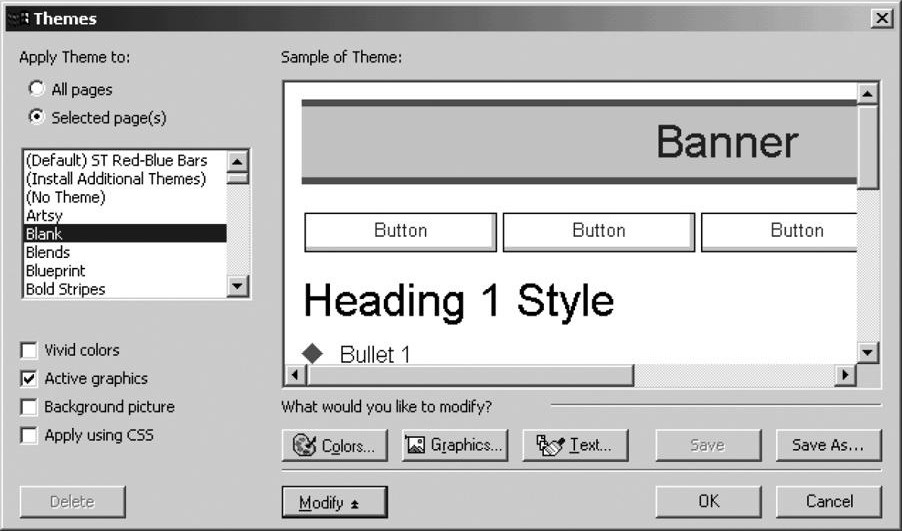
\includegraphics[width=0.6\textwidth]{MicrosoftFrontPage}
                    \caption{\centering Το γραφικό περιβάλλον του Microsoft FrontPage}
            \end{figure}

            Τα LCDPs που ακολούθησαν πήραν αυτές τις αρχές και τις εξέλιξαν, ενσωματώνοντας προηγμένα χαρακτηριστικά όπως η ευελιξία στη σύνδεση διαφορετικών συστημάτων, η χρήση cloud τεχνολογιών ή η υποστήριξη πολλαπλών πλατφορμών, δημιουργώντας εν τέλει εργαλεία που είναι ισχυρά, αλλά ταυτόχρονα προσιτά. \cite{LowCodeSimon}


    \section{Πλατφόρμες Ανάπτυξης Εφαρμογών σε Low-Code (LCDP)} \label{sec:LCDP}
        Όσο και αν η έννοια των μοντέλων άλλαξε τη μηχανική λογισμικού και έθεσε νέες προδιαγραφές στον σχεδιασμό του, η εξάρτησή της από δύσχρηστα πρότυπα όπως το UML περιόριζε την ευρεία υιοθέτησή της στη βιομηχανία. Ανταποκρινόμενες σε αυτή την πρόκληση, τα τελευταία χρόνια εμφανίστηκαν πλατφόρμες που αξιοποιούν τις αρχές της αφαίρεσης των μοντέλων, αλλά με μια πιο πρακτική και προσβάσιμη προσέγγιση. Αυτές οι πλατφόρμες εστιάζουν στην απλοποίηση της διαδικασίας ανάπτυξης λογισμικού, επιτρέποντας στους χρήστες να δημιουργούν εφαρμογές με ελάχιστη ή και καθόλου γραφή κώδικα.

        Οι συγκεκριμένες πλατφόρμες, γνωστές ως \textbf{Πλατφόρμες Ανάπτυξης Εφαρμογών σε Low-Code} (Low-Code Development Platforms -- LCDPs)\footnote{Εναλλακτικές ονομασίες είναι Low-Code Platforms (LCP), Low-Code Development Platforms (LCDP), ενώ η διαδικασία ανάπτυξης αναφέρεται ως Low-Code Software Development (LCSD). Η έννοια του Low-Code συχνά αναφέρεται και ως Χαμηλός Κώδικας.}, ενσωματώνουν γραφικά περιβάλλοντα εργασίας, προκαθορισμένα πρότυπα και αυτοματοποιημένα εργαλεία, με στόχο να μειώσουν την εξάρτηση από πολύπλοκα τεχνικά μέσα και να επιταχύνουν τον κύκλο ανάπτυξης λογισμικού.\cite{Bock2021}

        \begin{figure}[h!] \noindent \centering
                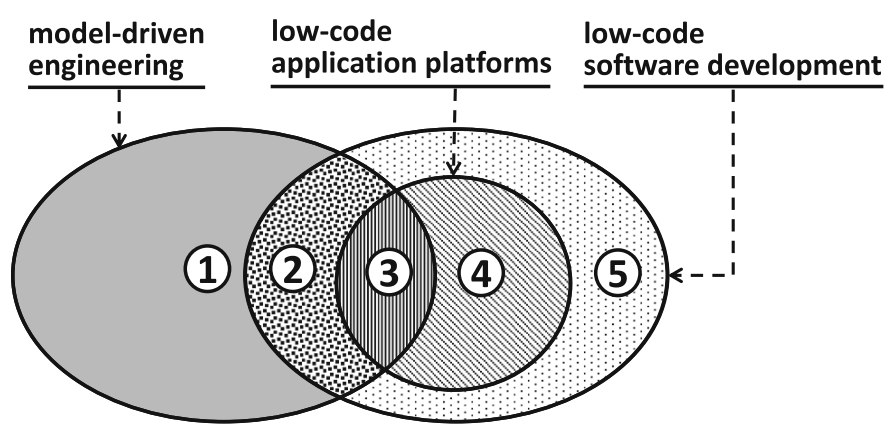
\includegraphics[width=0.6\textwidth]{MDE_LCSD}
                \caption{\centering Σύγκριση μεταξύ της μηχανικής που βασίζεται σε μοντέλα \\ και των Low-Code πλατφορμών. \cite{MDELow}}
                \label{fig:MDE_LCSD}
        \end{figure}

        Το σχήμα \ref{fig:MDE_LCSD} αποτυπώνει την αλληλεπίδραση και τις διαφορές μεταξύ της μηχανικής που βασίζεται σε μοντέλα (model-driven engineering), των πλατφορμών ανάπτυξης εφαρμογών σε low-code (low-code application platforms) και της ανάπτυξης λογισμικού σε low-code (low-code software development). Στην περιοχή 1, τα μοντέλα χρησιμοποιούνται χωρίς ιδιαίτερη έμφαση στη μείωση του κώδικα, αντικατοπτρίζοντας μια παραδοσιακή προσέγγιση στη μηχανική λογισμικού.
        Αντίθετα, στις περιοχές 2 και 3, οι προσπάθειες εστιάζουν στη μείωση του κώδικα, κάτι που αποτελεί κεντρικό στόχο των low-code πλατφορμών. Από την άλλη γίνεται να υπάρχουν προσπάθειες μείωσης κώδικα χωρίς να είναι απαραίτητη η χρήση μοντέλων (περιοχές 4 και 5), όπου οι πλατφόρμες συχνά βασίζονται σε άλλου είδους δομές, όπως δεδομένα από σχεσιακές βάσεις ή XML αρχεία. Μια κρίσιμη διαφοροποίηση μεταξύ των low-code application platforms και του low-code software development είναι ότι οι πλατφόρμες προσφέρουν πρόσθετα χαρακτηριστικά, όπως τη δυνατότητα διάθεσης του λογισμικού στο ευρύ κοινό και τη διαχείρισή του καθ' όλη τη διάρκεια του κύκλου ζωής του.

        \begin{figure}[h!] \noindent \centering
                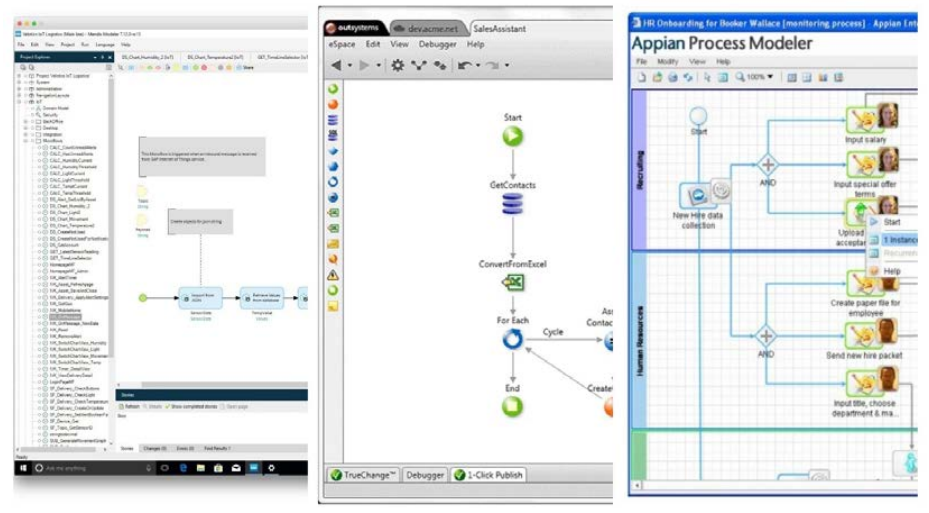
\includegraphics[width=0.9\textwidth]{LowCodePlatforms}
                \caption{Στιγμιότυπα από LCDP από αριστερά προς τα δεξιά: Mendix, OutSystems, Appian \cite{LowCodeMendix}}
        \end{figure}

        Μια \textbf{Πλατφόρμα Ανάπτυξης Εφαρμογών σε Low-Code} (LCDP) είναι μια πλατφόρμα ανάπτυξης λογισμικού που συνήθως λειτουργεί ως Platform-as-service (PaaS) βασιζόμενη στο clout και έχει σχεδιαστεί για να υποστηρίζει την ταχεία ανάπτυξη, εκτέλεση και διαχείριση εφαρμογών με ελάχιστο ή καθόλου ανάγκη για παραδοσιακό κώδικα και δομημένο προγραμματισμό. Αντίθετα, παρέχεται περιβάλλον με οπτικές αφαιρέσεις (visual abstractions) και χρησιμοποιείται προγραμματισμός με υψηλό επίπεδο αφαιρέσεων χρησιμοποιώντας μοντέλα και μεταδεδομένα.

        Η αποδοτική ανάπτυξη λογισμικού με χαμηλό κόστος και ελάχιστη προσπάθεια αποτελεί το βασικό στόχο των LCDP. Αυτές οι πλατφόρμες διευκολύνουν την γρήγορη προσαρμογή των εφαρμογών στις συνεχώς μεταβαλλόμενες τεχνολογικές ανάγκες και συνθήκες των σύγχρονων λειτουργικών συστημάτων. Με την εξαιρετική ευχέρεια προσαρμογής τους, οι οργανισμοί μπορούν να αντιδράσουν άμεσα στις απαιτήσεις της αγοράς, αναπτύσσοντας εφαρμογές που είναι συμβατές με νέες τεχνολογίες και νέες ανάγκες των χρηστών χωρίς να απαιτείται συνεχής αναθεώρηση του κώδικα.

        Η χρήση των LCDP έχει τύχει θετικής αποδοχής από τη βιομηχανία με πολλές εταιρείες και οργανισμοί να έχουν ενσωματώσει αυτές τις πλατφόρμες στις στρατηγικές τους για την ανάπτυξη λογισμικού και την υιοθέτησή τους συνεχώς να αυξάνεται. \cite{Bock2021,Bucaioni2022,Sahay2020}

        Οι τεχνολογίες των LCDP δεν είναι ούτε νέες, ούτε καινοτόμες. Αντίθετα, περιλαμβάνουν γνωστά εργαλεία και χαρακτηριστικά που χρησιμοποιούνται κατά κόρον εδώ και χρόνια σε κάποια μορφή. Το πλεονέκτημα όμως των LCDP είναι ότι συνδυάζουν αυτά τα εργαλεία και χαρακτηριστικά σε ένα ενιαίο περιβάλλον προσφέροντας μια ολοκληρωμένη λύση για την ανάπτυξη λογισμικού. Αυτό επιτρέπει στους χρήστες να αναπτύσσουν εφαρμογές με μεγάλη ταχύτητα, ενώ ταυτόχρονα διατηρούν την ευελιξία και την προσαρμοστικότητα που απαιτούνται από τις σύγχρονες εφαρμογές.

        \subsection{Χαρακτηριστικά και δομή των LCDP}
            Επιγραμματικά κάποια κοινά χαρακτηριστικά για τα οποία διακρίνονται οι Πλατφόρμες Ανάπτυξης Εφαρμογών σε Low-Code είναι τα εξής:

            \begin{itemize}[label={\tiny \blacksquare}]
                \setlength\itemsep{-0.25em}
                \item Γραφικός σχεδιαστής (GUI Designer): Ένα από τα πιο προφανή χαρακτηριστικά των LCDP είναι το γραφικό περιβάλλον χρήστη, ο οποίος παρέχει υποστήριξη για την προσαρμογή του GUI σε διαφορετικά περιβάλλοντα (υπολογιστές, κινητά κ.α.). Περιλαμβάνονται drag-and-drop εργαλεία, μηχανές αποφάσεων για τη μοντελοποίηση πολύπλοκης λογικής, κατασκευαστές φορμών (form builders) και άλλα.
                \item Μοντελοποίηση δομών δεδομένων: Σχεδόν πάντα εφαρμόζεται μια παραλλαγή του τυπικού μοντέλου οντοτήτων-συσχετίσεων (ER model). Σε ορισμένες περιπτώσεις οι δομές δεδομένων ορίζονται μόνο μέσω διαλόγων ή λιστών από το περιβάλλον διεπαφής του χρήστη. Συχνά υπάρχει πρόσβαση σε εξωτερικές πηγές δεδομένων χρησιμοποιώντας API και χρήση προτύπων όπως το JDBC\footnote{Java Database Connectivity: Πρότυπο για πρόσβαση σε βάσεις δεδομένων μέσω της Java.} και συνδέσμους (connectors) για άλλους τύπους αρχείων και συστημάτων. Τα δεδομένα σχεδιάζονται ώστε να αποθηκεύονται είτε στο εσωτερικό σύστημα βάσεων δεδομένων της πλατφόρμας είτε σε εξωτερικές πηγές.
                \item Ροή προγράμματος: Χρήση απλών γλωσσικών εκφράσεων για κανόνες απόφασης και καθορισμού συνθηκών ροής προγράμματος. Περιλαμβάνονται βιβλιοθήκες με λειτουργίες γενικού τύπου (όπως μαθηματικές συναρτήσεις) ή την ενσωμάτωση εσωτερικών λειτουργιών (για παράδειγμα REST υπηρεσίες).
                \item Φορητότητα και συνεργασία: Οι LCDP διευκολύνουν τη συνεργασία, επιτρέποντας στους χρήστες να εργάζονται από οποιαδήποτε τοποθεσία και συσκευή, ανεξαρτήτως λειτουργικού συστήματος.
                \item Επεκτασιμότητα: Η επαναχρησιμοποίηση προκατασκευασμένων στοιχείων μειώνει δραστικά τον χρόνο ανάπτυξης, ενώ η ύπαρξη marketplace επιτρέπει στους χρήστες να προσθέτουν νέα modules ή λειτουργίες στις εφαρμογές τους. Έτσι προσφέρεται η δυνατότητα εύκολης ενσωμάτωσης τρίτων modules, καθιστώντας τις εφαρμογές πιο ευέλικτες και προσαρμόσιμες στις ανάγκες των προγραμματιστών ή των τελικών χρηστών.
                \item Εύκολη διάθεση και έλεγχος έκδοσης: Ορισμένες πλατφόρμες η εφαρμογή να γίνεται deploy απομακρυσμένα σε κάποιον διακομιστή, ενώ άλλες το επιτρέπουν στο εκάστοτε μηχάνημα. Κάθε LCDP ενσωματώνει χαρακτηριστικά Dev Ops όπως το version control μέσω Git, διευκολύνοντας την παρακολούθηση αλλαγών και την αναίρεση ανεπιθύμητων ενεργειών. \cite{Bock2021}
            \end{itemize}

            Περνώντας σε παραπάνω λεπτομέρειες, αρχιτεκτονικά οι Πλατφόρμες Ανάπτυξης Λογισμικού σε Low-Code διαχωρίζονται σε τέσσερα επίπεδα: Το υψηλότερο επίπεδο, το \textit{Επίπεδο Εφαρμογής} (Application Layer) περιλαμβάνει το γραφικό περιβάλλον με το οποίο αλληλεπιδρούν οι χρήστες. Εκεί βρίσκονται τα εργαλεία και τα widgets που χρησιμοποιούνται για τη δημιουργία των σελίδων της εφαρμογής. Είναι το μέρος που οι χρήστες μπορούν να καθορίσουν τη συμπεριφορά της εφαρμογής, να συνδέσουν δεδομένα από εξωτερικές πηγές και να τα επεξεργαστούν και περιλαμβάνονται μηχανισμοί επαλήθευσης ταυτότητας και εξουσιοδότησης. Για τη σύνδεση των εξωτερικών πηγών μέσω των μηχανισμών επαλήθευσης ταυτότητας και των API (για παράδειγμα DropBox ή Git) χρησιμοποιείται το \textit{Επίπεδο Ενσωμάτωσης Υπηρεσιών} (Service Integration Layer). Αμέσως χαμηλότερα, το \textit{Επίπεδο Ενσωμάτωσης Δεδομένων} (Data Integration Layer) επιτρέπει την ομοιόμορφη διαχείρισης, επεξεργασία και ενοποίηση δεδομένων, ακόμα αν προέρχονται από ετερογενείς πηγές. Το χαμηλότερο επίπεδο είναι το \textit{Επίπεδο Διανομής} (Deployment Layer) στο οποίο η εκάστοτε εφαρμογή πακετάρεται και διανέμεται στο cloud. \cite{Sahay2020}

            \begin{figure}[h!] \noindent \centering
                    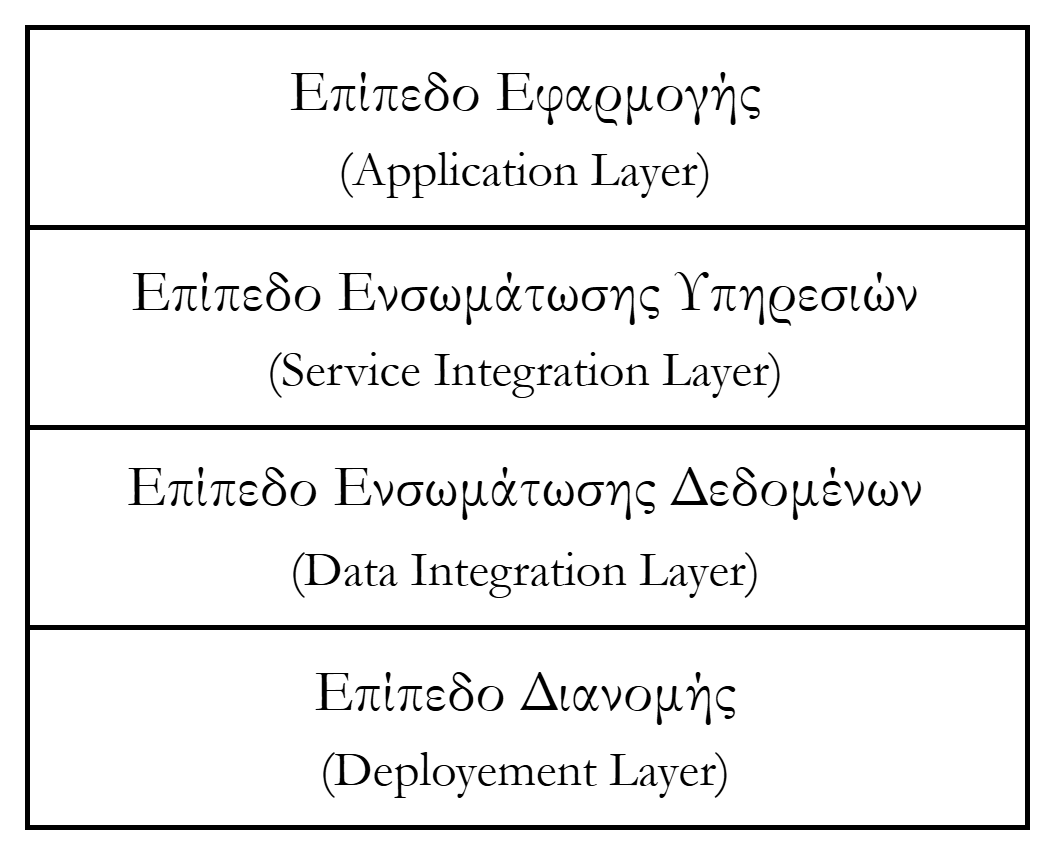
\includegraphics[width=0.4\textwidth]{diagrams/LCDP_ArchitectureLayers}
                    \caption{Αρχιτεκτονικός σχεδιασμός των LCDP \cite{Sahay2020}}
            \end{figure}

            Επεκτείνοντας την αρχιτεκτονική των τεσσάρων προαναφερθέντων επιπέδων, μπορούμε να ομαδοποιήσουμε τα κύρια στοιχεία που συνθέτουν οποιαδήποτε Πλατφόρμα Ανάπτυξης Λογισμικού σε Low-Code (LCDP) σε τρία μέρη: Το πρώτο μέρος περιλαμβάνει τον \textit{μοντελοποιητή εφαρμογών} (application modeler), το βασικό μηχανισμό που επιτρέπει στους χρήστες να δημιουργούν και να διαμορφώνουν εφαρμογές μέσω μιας γραφικής διεπαφής, το δεύτερο μέρος αφορά την πλευρά του \textit{διακομιστή} (server-side) (περιλαμβάνει τον κεντρικό μηχανισμό επεξεργασίας που χειρίζεται και επεξεργάζεται τα δεδομένα και διαχειρίζεται την ασφάλεια και επικοινωνία μεταξύ των εξωτερικών πηγών δεδομένων), ενώ το τρίτο μέρος επικεντρώνεται στις \textit{εξωτερικές υπηρεσίες} (external services) που ενσωματώνονται στην πλατφόρμα.

            Υπάρχει υποστήριξη και για SQL και για NoSQL βάσεις δεδομένων\footnote{Οι SQL βάσεις δεδομένων οργανώνουν τα δεδομένα σε πίνακες με γραμμές και στήλες όπου κάθε γραμμή αντιπροσωπεύει μια εγγραφή και κάθε στήλη ένα πεδίο δεδομένων. Οι NoSQL βάσεις δε χρησιμοποιούν αυτή την παραδοσιακή σχέση πίνακα-γραμμής-στήλης αλλά υποστηρίζουν διάφορους τύπους αποθήκευσης δεδομένων όπως έγγραφα, κλειδιά-τιμές ή γραφήματα και είναι πιο ευέλικτες στην επεξεργασία μη δομημένων δεδομένων.}. Όποιο και να είναι το είδος των δεδομένων, οι προγραμματιστές των εφαρμογών δεν χρειάζεται να ασχολούνται με τη διαχείριση των δεδομένων σε χαμηλό επίπεδο καθώς όλες οι διαδικασίες δημιουργίας, συντονισμού και διαχείρισης των δεδομένων πραγματοποιούνται στο back-end της πλατφόρμας. Επίσης, συνήθως παρέχονται αποθετήρια (repositories) για τη διαχείριση των εκδόσεων της εφαρμογής (version control), διευκολύνοντας τη συνεργασία μεταξύ των ομάδων ανάπτυξης και επιτρέποντας την παρακολούθηση και την ανάκτηση προηγούμενων εκδόσεων της εφαρμογής. Για να υποστηριχθεί η συνεργατική ανάπτυξη, οι LCDP ενσωματώνουν πλήθος εργαλείων και λειτουργιών που διευκολύνουν τη χρήση μεθοδολογιών ανάπτυξης λογισμικού, όπως το Agile, το Kanban και το Scrum. Αυτές οι μεθοδολογίες επιτρέπουν στις ομάδες ανάπτυξης να εργάζονται σε μικρότερα, διαχειρίσιμα κομμάτια του έργου, ενώ παράλληλα διευκολύνουν την επικοινωνία και τη συνεργασία. Μέσω αυτών των λειτουργιών, οι πλατφόρμες προσφέρουν ένα περιβάλλον που υποστηρίζει τη συνεχιζόμενη παράδοση (continuous delivery) και τη γρήγορη προσαρμογή στις αλλαγές των απαιτήσεων, κάτι που είναι καίριο για την ανάπτυξη σύγχρονων επιχειρηματικών εφαρμογών.

        \subsection{Διαδικασία ανάπτυξης στα LCDP}
            Για την ανάπτυξη μιας εφαρμογής μέσω πλατφορμών χαμηλού κώδικα (Low-Code Development Platforms – LCDPs), συνήθως ακολουθείται μια σειρά βημάτων που εξασφαλίζουν τη σωστή δομή και λειτουργικότητα της εφαρμογής. Το πρώτο βήμα περιλαμβάνει τη \textit{μοντελοποίηση δεδομένων}. Σε αυτή τη φάση, οι χρήστες χρησιμοποιούν το γραφικό περιβάλλον της πλατφόρμας για να διαμορφώσουν τις οντότητες της εφαρμογής, τις σχέσεις μεταξύ των οντοτήτων και να ορίσουν περιορισμούς και εξαρτήσεις. Αφού ολοκληρωθεί η μοντελοποίηση, ακολουθεί ο \textit{σχεδιασμός της διεπαφής χρήστη}. Σε αυτό το στάδιο, οι χρήστες διαμορφώνουν φόρμες και σελίδες που θα χρησιμοποιηθούν για την παρουσίαση της εφαρμογής. Παράλληλα, ορίζονται οι ρόλοι χρηστών και οι μηχανισμοί ασφαλείας που θα ισχύουν για τις οντότητες, τις φόρμες και τις σελίδες. Στη συνέχεια, γίνεται ο καθορισμός των κανόνων λογικής και των \textit{ροών εργασίας}. Αυτό περιλαμβάνει τη διαχείριση ροών μεταξύ φορμών ή σελίδων που απαιτούν διαφορετικές λειτουργίες, οι οποίες υλοποιούνται μέσω οπτικών ροών εργασίας. Ακολουθεί η \textit{ενσωμάτωση εξωτερικών υπηρεσιών} μέσω APIs τρίτων. Στο τελευταίο στάδιο γίνεται η \textit{διάθεση} της εφαρμογής, κάτι που μπορεί να γίνει στις περισσότερες πλατφόρμες με λίγα μόνο κλικ.

        \subsection{Παραδείγματα από (LCDP)}
            Όπως έχει αναφερθεί, οι πλατφόρμες ανάπτυξης εφαρμογών σε Low-Code έχουν γίνει δημοφιλείς στη βιομηχανία λογισμικού, με πολλές εταιρείες να επιλέγουν να χρησιμοποιούν αυτές τις πλατφόρμες για την ανάπτυξη των εφαρμογών τους. Κάποιες από τις πιο δημοφιλείς πλατφόρμες ανάπτυξης εφαρμογών σε Low-Code είναι η πλατφόρμα Mendix, η OutSystems και η σουίτα Power Apps της Microsoft.

            \subsubsection{Mendix}
            Το Mendix αποτελεί μια από τις κορυφαίες πλατφόρμες ανάπτυξης λογισμικού χαμηλού κώδικα, με drag-and-drop δυνατότητες και δυνατότητα για συνεργασία σε πραγματικό χρόνο με συναδέλφους με ενσωματωμένη χρήση Agile μεθόδων. Περιλαμβάνει γραφικό περιβάλλον που βοηθάει στην επαναχρησιμοποίηση διαφόρων στοιχείων κάτι που επιταχύνει τη διαδικασία ανάπτυξης, από τη ρύθμιση του μοντέλου δεδομένων ως τον ορισμό τνω διεπαφών χρήστη. Η πλατφόρμα υποστηρίζει ανάπτυξη εφαρμογών για web, mobile και PWA (Progressive Web Apps) και παρέχεται cloud υποδομή για άμεση διάθεση της εφαρμογής. Θα αναφερθούμε αναλυτικά στο Mendix στο κεφάλαιο \ref{ch:mendix}.

            \subsubsection{OutSystems}
            Η \textbf{OutSystems} είναι μια άλλη δημοφιλής PaaS βασισμένη στο cloud πλατφόρμα ανάπτυξης εφαρμογών χαμηλού κώδικα που είναι σχεδιασμένη με γνώμονα την απόδοση, την επεκτασιμότητα και την υψηλή διαθεσιμότητα. Αποτελεί ένα από τα κορυφαία ονόματα ειδικά στην ανάπτυξη mobile εφαρμογών, μαζί εταιρείες όπως η IBM, και η Gartner την χαρακτήρησε ως «οραματιστής» ανάμεσα σε 36 διαφορετικές πλατφόρμες ανάπτυξης mobile εφαρμογών. Τα πλεονεκτήματά της περιλαμβάνουν την προσέγγισή του που βασίζεται σε μοντέλα (model-driven approach) και τη συμπερίληψη μιας ποικιλίας APIs. Παρόλα αυτά, επισημάνθηκαν και κάποιες προειδοποιήσεις, όπως η έλλειψη ελέγχου στον παραγόμενο κώδικα, η ασυμβατότητα με τις παραδοσιακές μεθόδους ανάπτυξης και η απουσία ορισμένων επιλογών ανάπτυξης, τα οποία ενδέχεται να αποθαρρύνουν πιθανούς πελάτες από τη χρήση της πλατφόρμας. \cite{QuadrantOutSystems}

            \begin{figure}[h!] \noindent \centering
                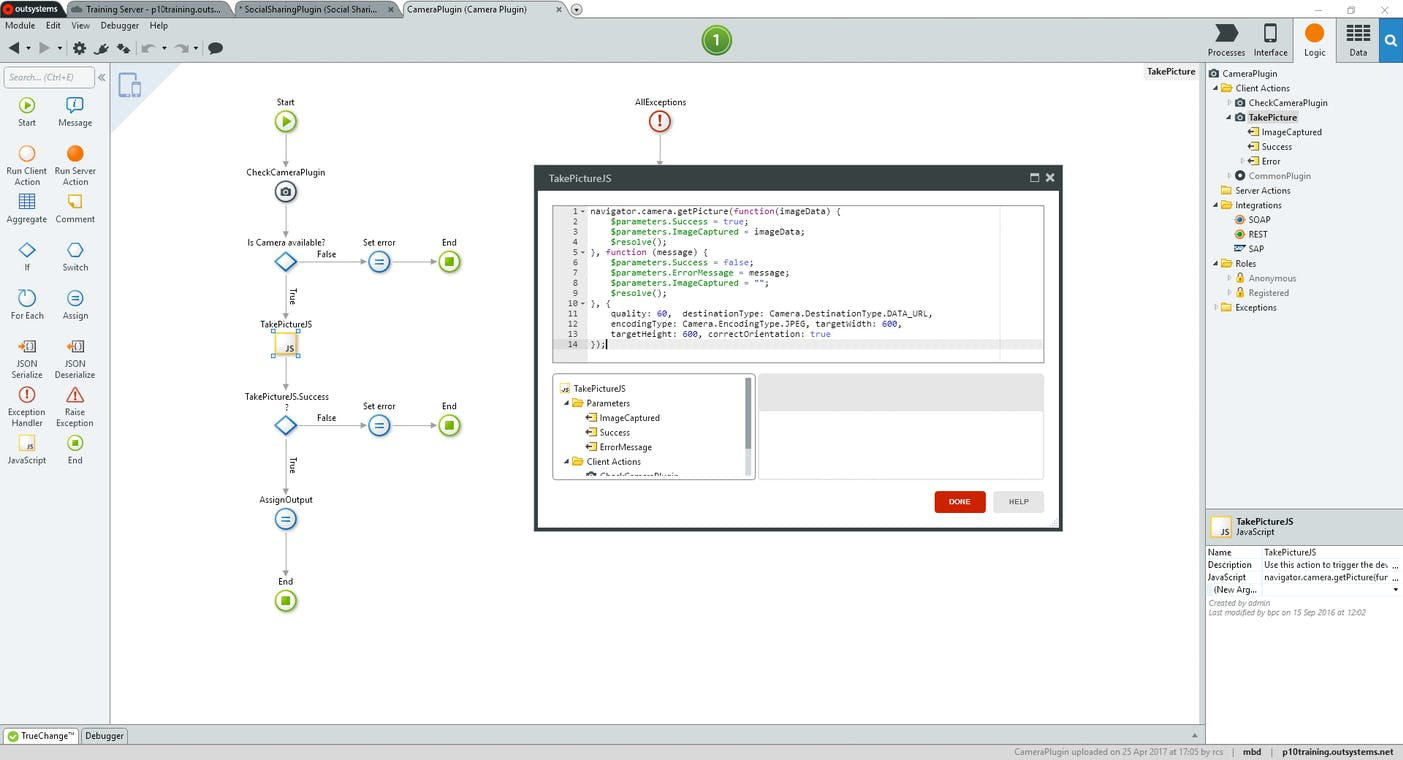
\includegraphics[width=0.8\textwidth]{OutSystemsScreenshot}
                \caption{\centering Στιγμιότυπο από τη πλατφόρμα OutSystems}
            \end{figure}

            Η πλατφόρμα αποτελείται από δύο μέρη: έναν διακομιστή και την αντίστοιχη εφαρμογή για υπολογιστές. Η εγκατάσταση του διακομιστή μπορεί να επεκταθεί με επιπλέον υπηρεσίες και αποθετήρια (repositories), αν αυτά είναι απαραίτητα για την ανάπτυξη των εφαρμογών. Για την ανάπτυξη των εφαρμογών μπορεί να χρησιμοποιηθούν περιβάλλοντα όπως το Microsoft .NET Stack ή το WebLogic της Oracle, και ο πηγαίος κώδικας των εφαρμογών παράγεται είτε σε C\# είτε σε Java, επιτρέποντας τη χρήση μηχανών όπως Common Language Runtime ή Java Virtual Machine. Η εφαρμογή της OutSystems, το Service Studio, δίνει εύκολη πρόσβαση σε όλες τις λειτουργίες της πλατφόρμας, όπως η μοντελοποίηση της διεπαφής χρήστη, τις βάσεις δεδομένων, SOAP/REST υπηρεσιών, προγραμματιζόμενων εργασιών κ.α. Πέρα από το Service Studio, διατίθεται και το Integration Studio, μια εφαρμογή επέκτασης της πλατφόρμας με πρόσθετη λειτουργικότητα, όπου οι προγραμματιστές μπορούν να ενοποιήσουν εξωτερικές βιβλιοθήκες, υπηρεσίες ή βάσεις δεδομένων με το OutSystems. Οι εφαρμογές Service Studio και το Integration Studio δεν εκτελούν τον κώδικα της πλατφόρμας τοπικά. Συνδέονται απομακρυσμένα στην OutSystems, επομένως δεν υπάρχουν μεγάλες απαιτήσεις σε υπολογιστική ισχύ ή σε διαθέσιμο αποθηκευτικό χώρο, παρά μόνο καλή σύνδεση στο διαδίκτυο, και επιπλέον είναι διαθέσιμες και σε browser μορφή, κάτι που εξαλείφει εντελώς την ανάγκη για εγκατάστασή τους. \cite{OutSystemsGolovin} \cite{OutSystemsSite}

            \subsubsection{Power Apps}
                Το \textbf{Power Apps} είναι μια άλλη PaaS πλατφόρμα για την ανάπτυξη εφαρμογών σε χαμηλό κώδικα. Σε αντίθεση με πλατφόρμες όπως την OutSystems που επικεντρώνεται στην ανάπτυξη εφαρμογών για καταναλωτές, όπως παιχνίδια ή mobile εφαρμογές ευρείας χρήσης, το Power Apps εστιάζει στην παροχή εργαλείων για τη δημιουργία προσαρμοσμένων λύσεων που ανταποκρίνονται στις εσωτερικές ανάγκες των επιχειρήσεων.

                \begin{figure}[h!] \noindent \centering
                        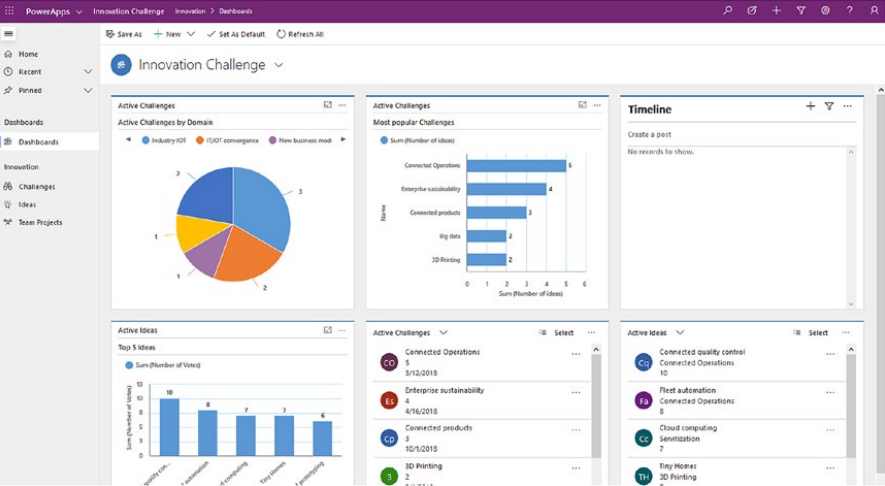
\includegraphics[width=0.8\textwidth]{PowerAppsSampleApp}
                        \caption{\centering Παράδειγμα portal app στο Power Apps}
                \end{figure}

                Η Microsoft παρουσίασε το \textbf{Power Apps} στα τέλη του 2016, προσφέροντας ένα γραφικό περιβάλλον χρήστη που θύμιζε έντονα εκείνο του Microsoft Excel, διευκολύνοντας έτσι τους χρήστες με βασικές γνώσεις του οικοσυστήματος της εταιρείας να προσαρμοστούν γρήγορα. Από την αρχή, το Power Apps υποστήριζε την ενσωμάτωση δεδομένων από διάφορες πηγές, όπως το SharePoint, το Dynamics 365, οι διακομιστές SQL και εκατοντάδες ακόμη συνδέσεις, ενισχύοντας τη χρησιμότητά του για οργανισμούς με διαφορετικές ανάγκες δεδομένων. Στα επόμενα χρόνια, η πλατφόρμα εξελίχθηκε περαιτέρω με την εισαγωγή ενός νέου τρόπου ανάπτυξης εφαρμογών βασισμένου σε μοντέλα (model-driven development) ο οποίος επέτρεψε τη δημιουργία λειτουργικών διεπαφών χρήστη με ελάχιστη ή και καθόλου παρέμβαση από προγραμματιστές. Το 2019, η Microsoft εισήγαγε τα Power Apps Portals, μια υπηρεσία που επέτρεπε τη δημιουργία ιστοσελίδων. Αυτή η προσθήκη ενίσχυσε σημαντικά τις δυνατότητες του Power Apps, καθώς πλέον οι επιχειρήσεις μπορούσαν να δημιουργήσουν ιστοσελίδες που επιτρέπουν σε χρήστες εκτός της επιχείρησης να έχουν πρόσβαση στις επιχειρηματικές εφαρμογές τους. \cite{PowerAppsLeung}
